% Options for packages loaded elsewhere
\PassOptionsToPackage{unicode}{hyperref}
\PassOptionsToPackage{hyphens}{url}
%
\documentclass[
]{article}
\usepackage{amsmath,amssymb}
\usepackage{lmodern}
\usepackage{iftex}
\ifPDFTeX
  \usepackage[T1]{fontenc}
  \usepackage[utf8]{inputenc}
  \usepackage{textcomp} % provide euro and other symbols
\else % if luatex or xetex
  \usepackage{unicode-math}
  \defaultfontfeatures{Scale=MatchLowercase}
  \defaultfontfeatures[\rmfamily]{Ligatures=TeX,Scale=1}
\fi
% Use upquote if available, for straight quotes in verbatim environments
\IfFileExists{upquote.sty}{\usepackage{upquote}}{}
\IfFileExists{microtype.sty}{% use microtype if available
  \usepackage[]{microtype}
  \UseMicrotypeSet[protrusion]{basicmath} % disable protrusion for tt fonts
}{}
\makeatletter
\@ifundefined{KOMAClassName}{% if non-KOMA class
  \IfFileExists{parskip.sty}{%
    \usepackage{parskip}
  }{% else
    \setlength{\parindent}{0pt}
    \setlength{\parskip}{6pt plus 2pt minus 1pt}}
}{% if KOMA class
  \KOMAoptions{parskip=half}}
\makeatother
\usepackage{xcolor}
\IfFileExists{xurl.sty}{\usepackage{xurl}}{} % add URL line breaks if available
\IfFileExists{bookmark.sty}{\usepackage{bookmark}}{\usepackage{hyperref}}
\hypersetup{
  pdftitle={lab1},
  pdfauthor={Suschevskiy Vsevolod},
  hidelinks,
  pdfcreator={LaTeX via pandoc}}
\urlstyle{same} % disable monospaced font for URLs
\usepackage[margin=1in]{geometry}
\usepackage{color}
\usepackage{fancyvrb}
\newcommand{\VerbBar}{|}
\newcommand{\VERB}{\Verb[commandchars=\\\{\}]}
\DefineVerbatimEnvironment{Highlighting}{Verbatim}{commandchars=\\\{\}}
% Add ',fontsize=\small' for more characters per line
\usepackage{framed}
\definecolor{shadecolor}{RGB}{248,248,248}
\newenvironment{Shaded}{\begin{snugshade}}{\end{snugshade}}
\newcommand{\AlertTok}[1]{\textcolor[rgb]{0.94,0.16,0.16}{#1}}
\newcommand{\AnnotationTok}[1]{\textcolor[rgb]{0.56,0.35,0.01}{\textbf{\textit{#1}}}}
\newcommand{\AttributeTok}[1]{\textcolor[rgb]{0.77,0.63,0.00}{#1}}
\newcommand{\BaseNTok}[1]{\textcolor[rgb]{0.00,0.00,0.81}{#1}}
\newcommand{\BuiltInTok}[1]{#1}
\newcommand{\CharTok}[1]{\textcolor[rgb]{0.31,0.60,0.02}{#1}}
\newcommand{\CommentTok}[1]{\textcolor[rgb]{0.56,0.35,0.01}{\textit{#1}}}
\newcommand{\CommentVarTok}[1]{\textcolor[rgb]{0.56,0.35,0.01}{\textbf{\textit{#1}}}}
\newcommand{\ConstantTok}[1]{\textcolor[rgb]{0.00,0.00,0.00}{#1}}
\newcommand{\ControlFlowTok}[1]{\textcolor[rgb]{0.13,0.29,0.53}{\textbf{#1}}}
\newcommand{\DataTypeTok}[1]{\textcolor[rgb]{0.13,0.29,0.53}{#1}}
\newcommand{\DecValTok}[1]{\textcolor[rgb]{0.00,0.00,0.81}{#1}}
\newcommand{\DocumentationTok}[1]{\textcolor[rgb]{0.56,0.35,0.01}{\textbf{\textit{#1}}}}
\newcommand{\ErrorTok}[1]{\textcolor[rgb]{0.64,0.00,0.00}{\textbf{#1}}}
\newcommand{\ExtensionTok}[1]{#1}
\newcommand{\FloatTok}[1]{\textcolor[rgb]{0.00,0.00,0.81}{#1}}
\newcommand{\FunctionTok}[1]{\textcolor[rgb]{0.00,0.00,0.00}{#1}}
\newcommand{\ImportTok}[1]{#1}
\newcommand{\InformationTok}[1]{\textcolor[rgb]{0.56,0.35,0.01}{\textbf{\textit{#1}}}}
\newcommand{\KeywordTok}[1]{\textcolor[rgb]{0.13,0.29,0.53}{\textbf{#1}}}
\newcommand{\NormalTok}[1]{#1}
\newcommand{\OperatorTok}[1]{\textcolor[rgb]{0.81,0.36,0.00}{\textbf{#1}}}
\newcommand{\OtherTok}[1]{\textcolor[rgb]{0.56,0.35,0.01}{#1}}
\newcommand{\PreprocessorTok}[1]{\textcolor[rgb]{0.56,0.35,0.01}{\textit{#1}}}
\newcommand{\RegionMarkerTok}[1]{#1}
\newcommand{\SpecialCharTok}[1]{\textcolor[rgb]{0.00,0.00,0.00}{#1}}
\newcommand{\SpecialStringTok}[1]{\textcolor[rgb]{0.31,0.60,0.02}{#1}}
\newcommand{\StringTok}[1]{\textcolor[rgb]{0.31,0.60,0.02}{#1}}
\newcommand{\VariableTok}[1]{\textcolor[rgb]{0.00,0.00,0.00}{#1}}
\newcommand{\VerbatimStringTok}[1]{\textcolor[rgb]{0.31,0.60,0.02}{#1}}
\newcommand{\WarningTok}[1]{\textcolor[rgb]{0.56,0.35,0.01}{\textbf{\textit{#1}}}}
\usepackage{graphicx}
\makeatletter
\def\maxwidth{\ifdim\Gin@nat@width>\linewidth\linewidth\else\Gin@nat@width\fi}
\def\maxheight{\ifdim\Gin@nat@height>\textheight\textheight\else\Gin@nat@height\fi}
\makeatother
% Scale images if necessary, so that they will not overflow the page
% margins by default, and it is still possible to overwrite the defaults
% using explicit options in \includegraphics[width, height, ...]{}
\setkeys{Gin}{width=\maxwidth,height=\maxheight,keepaspectratio}
% Set default figure placement to htbp
\makeatletter
\def\fps@figure{htbp}
\makeatother
\setlength{\emergencystretch}{3em} % prevent overfull lines
\providecommand{\tightlist}{%
  \setlength{\itemsep}{0pt}\setlength{\parskip}{0pt}}
\setcounter{secnumdepth}{-\maxdimen} % remove section numbering
\ifLuaTeX
  \usepackage{selnolig}  % disable illegal ligatures
\fi

\title{lab1}
\author{Suschevskiy Vsevolod}
\date{2022-05-09}

\begin{document}
\maketitle

\hypertarget{basics}{%
\subsection{basics}\label{basics}}

\begin{Shaded}
\begin{Highlighting}[]
\FunctionTok{library}\NormalTok{(tidyverse)}
\end{Highlighting}
\end{Shaded}

\begin{verbatim}
## -- Attaching packages --------------------------------------- tidyverse 1.3.1 --
\end{verbatim}

\begin{verbatim}
## v ggplot2 3.3.5     v purrr   0.3.4
## v tibble  3.1.6     v dplyr   1.0.8
## v tidyr   1.2.0     v stringr 1.4.0
## v readr   2.1.2     v forcats 0.5.1
\end{verbatim}

\begin{verbatim}
## -- Conflicts ------------------------------------------ tidyverse_conflicts() --
## x dplyr::filter() masks stats::filter()
## x dplyr::lag()    masks stats::lag()
\end{verbatim}

\begin{figure}
\centering
\includegraphics{https://miro.medium.com/max/1400/1*mcLnnVdHNg-ikDbHJfHDNA.png}
\caption{components}
\end{figure}

\hypertarget{data}{%
\subsection{Data}\label{data}}

What is this dataset?

How familiar are your with mtcars?

Do you hate them?

\begin{Shaded}
\begin{Highlighting}[]
\NormalTok{?mtcars}
\end{Highlighting}
\end{Shaded}

\begin{Shaded}
\begin{Highlighting}[]
\NormalTok{mtcars }\SpecialCharTok{|}\ErrorTok{\textgreater{}} 
  \FunctionTok{head}\NormalTok{()}
\end{Highlighting}
\end{Shaded}

\begin{verbatim}
##                    mpg cyl disp  hp drat    wt  qsec vs am gear carb
## Mazda RX4         21.0   6  160 110 3.90 2.620 16.46  0  1    4    4
## Mazda RX4 Wag     21.0   6  160 110 3.90 2.875 17.02  0  1    4    4
## Datsun 710        22.8   4  108  93 3.85 2.320 18.61  1  1    4    1
## Hornet 4 Drive    21.4   6  258 110 3.08 3.215 19.44  1  0    3    1
## Hornet Sportabout 18.7   8  360 175 3.15 3.440 17.02  0  0    3    2
## Valiant           18.1   6  225 105 2.76 3.460 20.22  1  0    3    1
\end{verbatim}

\hypertarget{base-recap}{%
\subsection{base recap}\label{base-recap}}

\hypertarget{dimensions-of-data}{%
\subsubsection{dimensions of data}\label{dimensions-of-data}}

Lets warm up your R (tydyverse) skills and make use of Nastay's lecture

\begin{Shaded}
\begin{Highlighting}[]
\NormalTok{mtcars }\SpecialCharTok{|}\ErrorTok{\textgreater{}} 
\FunctionTok{ggplot}\NormalTok{(}\FunctionTok{aes}\NormalTok{(}\AttributeTok{x  =}\NormalTok{wt, }\AttributeTok{y =}\NormalTok{ mpg)) }\SpecialCharTok{+}
  \FunctionTok{geom\_point}\NormalTok{()}\SpecialCharTok{+}
  \FunctionTok{ggtitle}\NormalTok{(}\StringTok{"2 D"}\NormalTok{)}\SpecialCharTok{+}
  \FunctionTok{theme\_minimal}\NormalTok{()}
\end{Highlighting}
\end{Shaded}

\includegraphics{lab1_files/figure-latex/unnamed-chunk-4-1.pdf}

What is wrong with the following visualization?

\begin{Shaded}
\begin{Highlighting}[]
\NormalTok{mtcars }\SpecialCharTok{|}\ErrorTok{\textgreater{}} 
\FunctionTok{ggplot}\NormalTok{(}\FunctionTok{aes}\NormalTok{(}\AttributeTok{x  =}\NormalTok{wt, }\AttributeTok{y =}\NormalTok{ mpg, }\AttributeTok{color =}\NormalTok{ gear)) }\SpecialCharTok{+}
  \FunctionTok{geom\_point}\NormalTok{()}\SpecialCharTok{+}
  \FunctionTok{ggtitle}\NormalTok{(}\StringTok{"3 D, continious?"}\NormalTok{)}\SpecialCharTok{+}
  \FunctionTok{theme\_minimal}\NormalTok{()}
\end{Highlighting}
\end{Shaded}

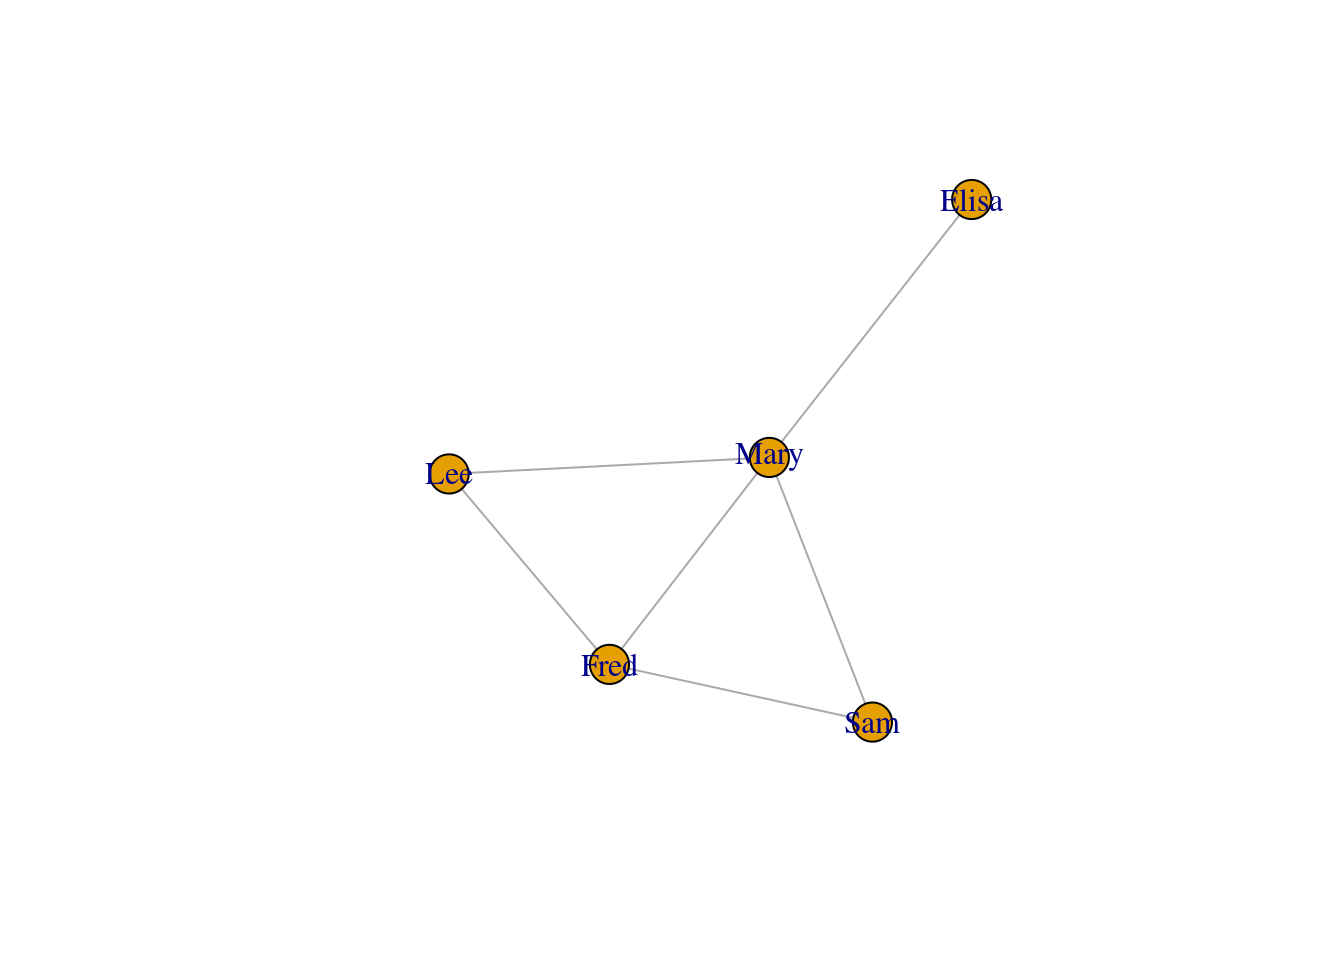
\includegraphics{lab1_files/figure-latex/unnamed-chunk-5-1.pdf}

What is the difference between categorical variable and factor?

\begin{Shaded}
\begin{Highlighting}[]
\NormalTok{mtcars }\SpecialCharTok{|}\ErrorTok{\textgreater{}} 
\FunctionTok{ggplot}\NormalTok{(}\FunctionTok{aes}\NormalTok{(}\AttributeTok{x  =}\NormalTok{wt, }\AttributeTok{y =}\NormalTok{ mpg, }\AttributeTok{color =}\NormalTok{ gear }\SpecialCharTok{|}\ErrorTok{\textgreater{}} \FunctionTok{as\_factor}\NormalTok{())) }\SpecialCharTok{+}
  \FunctionTok{geom\_point}\NormalTok{()}\SpecialCharTok{+}
  \FunctionTok{ggtitle}\NormalTok{(}\StringTok{"3 D"}\NormalTok{)}\SpecialCharTok{+}
  \FunctionTok{theme\_minimal}\NormalTok{()}
\end{Highlighting}
\end{Shaded}

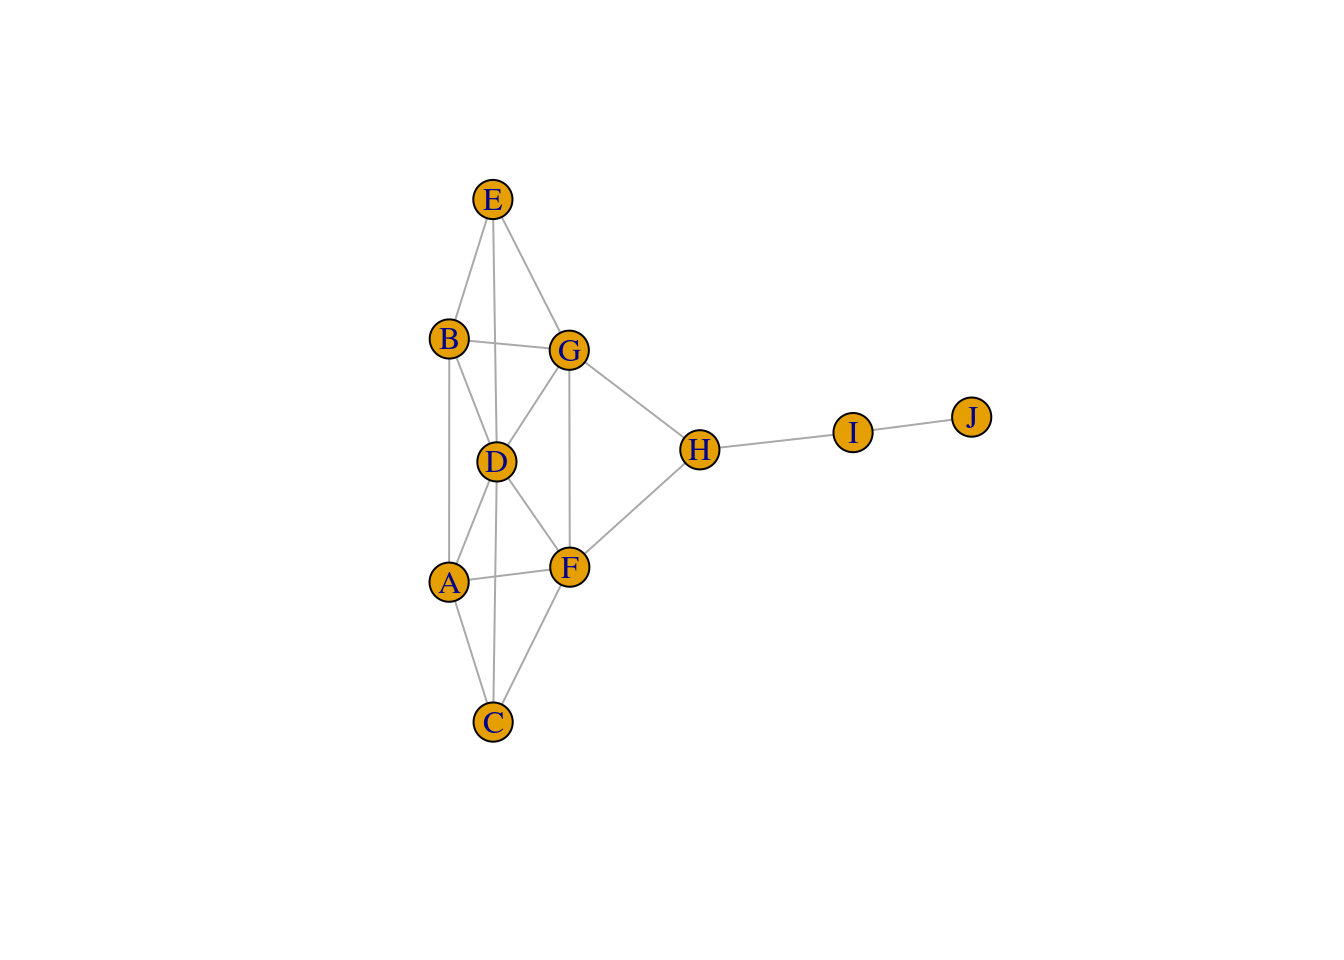
\includegraphics{lab1_files/figure-latex/unnamed-chunk-6-1.pdf}

How easy is to read the following graph?

\begin{Shaded}
\begin{Highlighting}[]
\NormalTok{mtcars }\SpecialCharTok{|}\ErrorTok{\textgreater{}} 
\FunctionTok{ggplot}\NormalTok{(}\FunctionTok{aes}\NormalTok{(}\AttributeTok{x  =}\NormalTok{wt, }\AttributeTok{y =}\NormalTok{ mpg, }
           \AttributeTok{color =}\NormalTok{ gear }\SpecialCharTok{|}\ErrorTok{\textgreater{}} \FunctionTok{as\_factor}\NormalTok{(),}
           \AttributeTok{size =}\NormalTok{ cyl)) }\SpecialCharTok{+}
  \FunctionTok{geom\_point}\NormalTok{()}\SpecialCharTok{+}
  \FunctionTok{ggtitle}\NormalTok{(}\StringTok{"4 D"}\NormalTok{)}\SpecialCharTok{+}
  \FunctionTok{theme\_minimal}\NormalTok{()}
\end{Highlighting}
\end{Shaded}

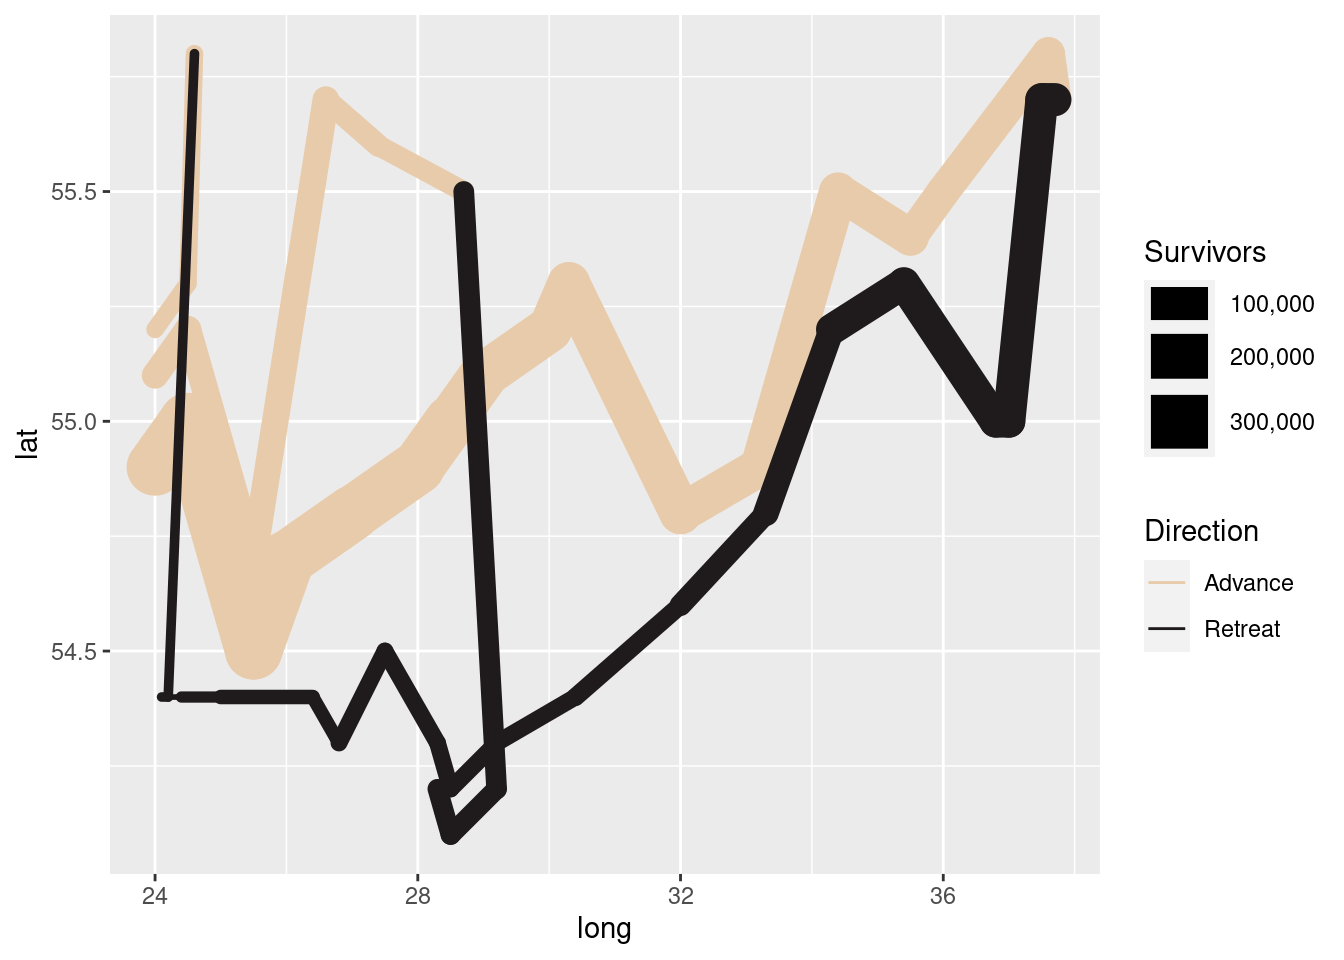
\includegraphics{lab1_files/figure-latex/unnamed-chunk-7-1.pdf}

What is the difference between these two graphs? How different will be
your story?

\begin{Shaded}
\begin{Highlighting}[]
\NormalTok{mtcars }\SpecialCharTok{|}\ErrorTok{\textgreater{}} 
\FunctionTok{ggplot}\NormalTok{(}\FunctionTok{aes}\NormalTok{(}\AttributeTok{x =}\NormalTok{wt, }\AttributeTok{y =}\NormalTok{ mpg, }
           \AttributeTok{color =}\NormalTok{ gear }\SpecialCharTok{|}\ErrorTok{\textgreater{}} \FunctionTok{as\_factor}\NormalTok{(),}
           \AttributeTok{size =}\NormalTok{ cyl }\SpecialCharTok{|}\ErrorTok{\textgreater{}} \FunctionTok{as.factor}\NormalTok{())) }\SpecialCharTok{+}
  \FunctionTok{geom\_point}\NormalTok{()}\SpecialCharTok{+}
  \FunctionTok{facet\_wrap}\NormalTok{(}\SpecialCharTok{\textasciitilde{}}\NormalTok{cyl)}\SpecialCharTok{+} 
  \FunctionTok{ggtitle}\NormalTok{(}\StringTok{"4 D"}\NormalTok{, }\StringTok{"distinct by Number of cylinders"}\NormalTok{)}\SpecialCharTok{+}
  \FunctionTok{theme\_minimal}\NormalTok{()}
\end{Highlighting}
\end{Shaded}

\begin{verbatim}
## Warning: Using size for a discrete variable is not advised.
\end{verbatim}

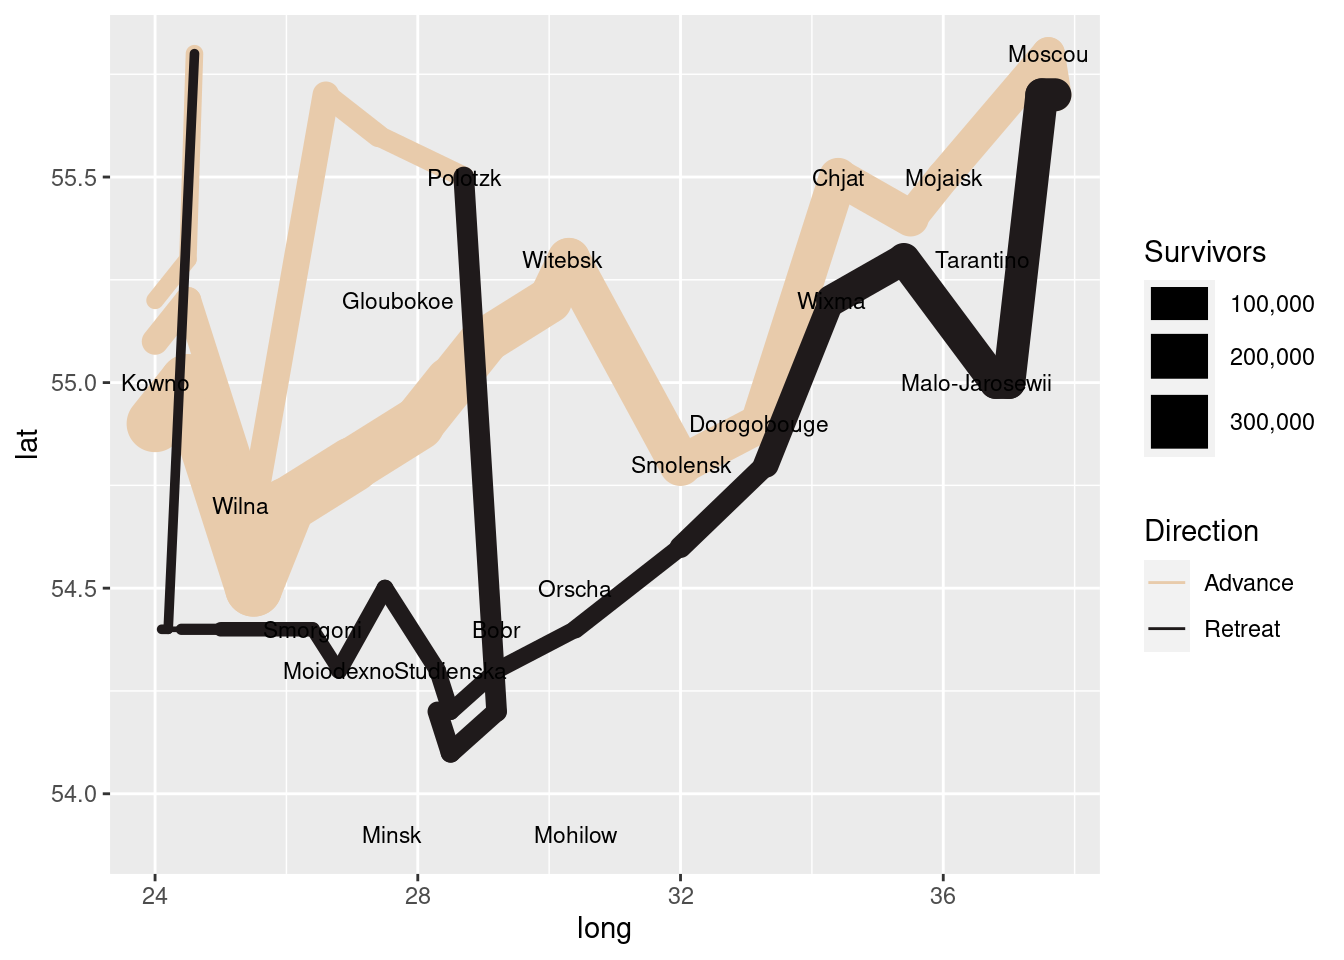
\includegraphics{lab1_files/figure-latex/unnamed-chunk-8-1.pdf}

Try to fix this on you own

\begin{Shaded}
\begin{Highlighting}[]
\NormalTok{mtcars }\SpecialCharTok{|}\ErrorTok{\textgreater{}} 
\FunctionTok{ggplot}\NormalTok{(}\FunctionTok{aes}\NormalTok{(}\AttributeTok{x =}\NormalTok{wt, }\AttributeTok{y =}\NormalTok{ mpg, }
           \AttributeTok{color =}\NormalTok{ gear }\SpecialCharTok{|}\ErrorTok{\textgreater{}} \FunctionTok{as\_factor}\NormalTok{(),}
           \AttributeTok{size =}\NormalTok{ cyl }\SpecialCharTok{|}\ErrorTok{\textgreater{}} \FunctionTok{as.factor}\NormalTok{())) }\SpecialCharTok{+}
  \FunctionTok{geom\_point}\NormalTok{()}\SpecialCharTok{+}
  \FunctionTok{stat\_smooth}\NormalTok{(}\AttributeTok{method=}\StringTok{\textquotesingle{}lm\textquotesingle{}}\NormalTok{)}\SpecialCharTok{+}
  \FunctionTok{facet\_wrap}\NormalTok{(}\SpecialCharTok{\textasciitilde{}}\NormalTok{cyl)}\SpecialCharTok{+}
  \FunctionTok{ggtitle}\NormalTok{(}\StringTok{"4 D"}\NormalTok{, }\StringTok{"with statistics, but something is wrong"}\NormalTok{)}\SpecialCharTok{+}
  \FunctionTok{theme\_minimal}\NormalTok{()}
\end{Highlighting}
\end{Shaded}

\begin{verbatim}
## Warning: Using size for a discrete variable is not advised.
\end{verbatim}

\begin{verbatim}
## `geom_smooth()` using formula 'y ~ x'
\end{verbatim}

\begin{verbatim}
## Warning in qt((1 - level)/2, df): NaNs produced
\end{verbatim}

\begin{verbatim}
## Warning in qt((1 - level)/2, df): NaNs produced

## Warning in qt((1 - level)/2, df): NaNs produced
\end{verbatim}

\begin{verbatim}
## Warning in max(ids, na.rm = TRUE): no non-missing arguments to max; returning
## -Inf

## Warning in max(ids, na.rm = TRUE): no non-missing arguments to max; returning
## -Inf

## Warning in max(ids, na.rm = TRUE): no non-missing arguments to max; returning
## -Inf
\end{verbatim}

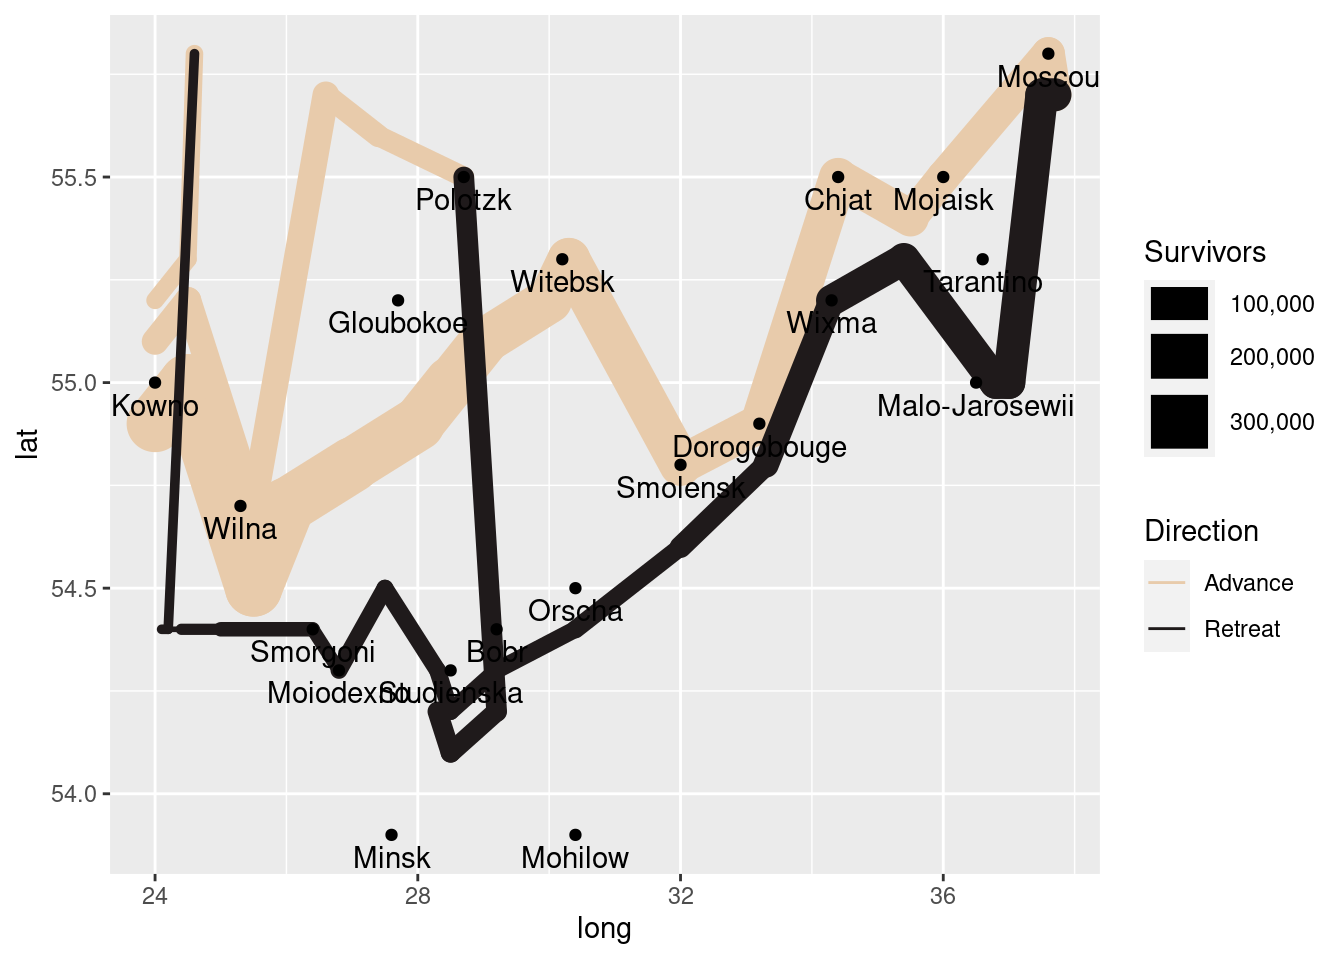
\includegraphics{lab1_files/figure-latex/unnamed-chunk-9-1.pdf}

Or look at the solution right away

What is the goal for adding statistics on graphs?

\begin{Shaded}
\begin{Highlighting}[]
\NormalTok{mtcars }\SpecialCharTok{|}\ErrorTok{\textgreater{}} 
\FunctionTok{ggplot}\NormalTok{(}\FunctionTok{aes}\NormalTok{(}\AttributeTok{x =}\NormalTok{wt, }\AttributeTok{y =}\NormalTok{ mpg, }
           \AttributeTok{color =}\NormalTok{ gear }\SpecialCharTok{|}\ErrorTok{\textgreater{}} \FunctionTok{as\_factor}\NormalTok{())) }\SpecialCharTok{+}
    \FunctionTok{geom\_smooth}\NormalTok{(}\AttributeTok{method=}\StringTok{\textquotesingle{}lm\textquotesingle{}}\NormalTok{)}\SpecialCharTok{+}
  \FunctionTok{geom\_point}\NormalTok{(}\FunctionTok{aes}\NormalTok{(}\AttributeTok{size =}\NormalTok{ cyl }\SpecialCharTok{|}\ErrorTok{\textgreater{}} \FunctionTok{as.factor}\NormalTok{()))}\SpecialCharTok{+}
  \CommentTok{\# facet\_wrap(\textasciitilde{}cyl)+}
  \FunctionTok{ggtitle}\NormalTok{(}\StringTok{"4 D"}\NormalTok{, }\StringTok{"with statistics"}\NormalTok{)}\SpecialCharTok{+}
  \FunctionTok{theme\_minimal}\NormalTok{()}
\end{Highlighting}
\end{Shaded}

\begin{verbatim}
## Warning: Using size for a discrete variable is not advised.
\end{verbatim}

\begin{verbatim}
## `geom_smooth()` using formula 'y ~ x'
\end{verbatim}

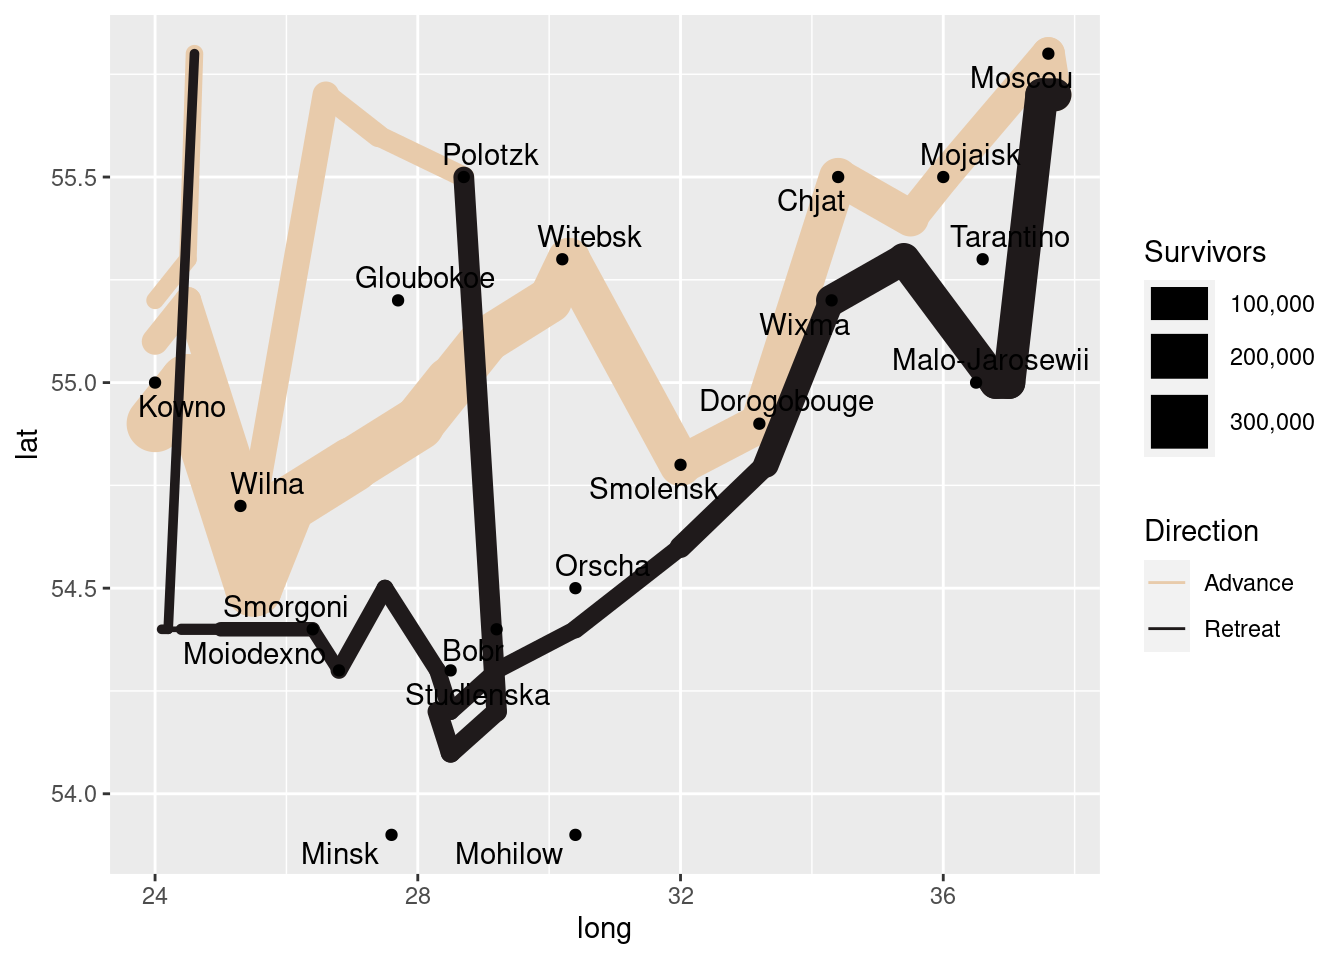
\includegraphics{lab1_files/figure-latex/unnamed-chunk-10-1.pdf}

Complex layers could be made of simpler one, thus giving us more
customization

\begin{Shaded}
\begin{Highlighting}[]
\NormalTok{mtcars }\SpecialCharTok{|}\ErrorTok{\textgreater{}} 
\FunctionTok{ggplot}\NormalTok{(}\FunctionTok{aes}\NormalTok{(}\AttributeTok{x =}\NormalTok{wt, }\AttributeTok{y =}\NormalTok{ mpg, }
           \AttributeTok{color =}\NormalTok{ gear }\SpecialCharTok{|}\ErrorTok{\textgreater{}} \FunctionTok{as\_factor}\NormalTok{())) }\SpecialCharTok{+}
  \FunctionTok{geom\_smooth}\NormalTok{(}\AttributeTok{method=}\StringTok{\textquotesingle{}lm\textquotesingle{}}\NormalTok{, }\AttributeTok{alpha =} \FloatTok{0.1}\NormalTok{, }\AttributeTok{size =} \DecValTok{0}\NormalTok{)}\SpecialCharTok{+}
  \FunctionTok{geom\_line}\NormalTok{(}\AttributeTok{stat=}\StringTok{"smooth"}\NormalTok{,}\AttributeTok{method =} \StringTok{"lm"}\NormalTok{, }\AttributeTok{size  =} \FloatTok{1.5}\NormalTok{, }\AttributeTok{alpha =} \FloatTok{0.5}\NormalTok{)}\SpecialCharTok{+}
  \FunctionTok{geom\_point}\NormalTok{(}\FunctionTok{aes}\NormalTok{(}\AttributeTok{size =}\NormalTok{ cyl }\SpecialCharTok{|}\ErrorTok{\textgreater{}} \FunctionTok{as.factor}\NormalTok{()))}\SpecialCharTok{+}
  \FunctionTok{ggtitle}\NormalTok{(}\StringTok{"4 D"}\NormalTok{, }\StringTok{"with statistics from basic attributes"}\NormalTok{)}\SpecialCharTok{+}
  \FunctionTok{theme\_minimal}\NormalTok{()}
\end{Highlighting}
\end{Shaded}

\begin{verbatim}
## Warning: Using size for a discrete variable is not advised.
\end{verbatim}

\begin{verbatim}
## `geom_smooth()` using formula 'y ~ x'
## `geom_smooth()` using formula 'y ~ x'
\end{verbatim}

\includegraphics{lab1_files/figure-latex/unnamed-chunk-11-1.pdf}

\hypertarget{colors}{%
\subsubsection{colors!}\label{colors}}

\begin{Shaded}
\begin{Highlighting}[]
\NormalTok{mtcars }\SpecialCharTok{|}\ErrorTok{\textgreater{}} 
\FunctionTok{ggplot}\NormalTok{(}\FunctionTok{aes}\NormalTok{(}\AttributeTok{x =}\NormalTok{wt, }\AttributeTok{y =}\NormalTok{ mpg, }
           \AttributeTok{color =}\NormalTok{ gear }\SpecialCharTok{|}\ErrorTok{\textgreater{}} \FunctionTok{as\_factor}\NormalTok{())) }\SpecialCharTok{+}
  \FunctionTok{geom\_smooth}\NormalTok{(}\AttributeTok{method=}\StringTok{\textquotesingle{}lm\textquotesingle{}}\NormalTok{, }\AttributeTok{alpha =} \FloatTok{0.1}\NormalTok{, }\AttributeTok{size =} \DecValTok{0}\NormalTok{)}\SpecialCharTok{+}
  \FunctionTok{geom\_line}\NormalTok{(}\AttributeTok{stat=}\StringTok{"smooth"}\NormalTok{,}\AttributeTok{method =} \StringTok{"lm"}\NormalTok{, }\AttributeTok{size  =} \FloatTok{1.5}\NormalTok{, }\AttributeTok{alpha =} \FloatTok{0.5}\NormalTok{)}\SpecialCharTok{+}
  \FunctionTok{geom\_point}\NormalTok{(}\FunctionTok{aes}\NormalTok{(}\AttributeTok{size =}\NormalTok{ cyl }\SpecialCharTok{|}\ErrorTok{\textgreater{}} \FunctionTok{as.factor}\NormalTok{()))}\SpecialCharTok{+}
  \FunctionTok{ggtitle}\NormalTok{(}\StringTok{"4 D"}\NormalTok{, }\StringTok{"with statistics from basic attributes"}\NormalTok{)}\SpecialCharTok{+}
  \FunctionTok{scale\_color\_brewer}\NormalTok{(}\AttributeTok{palette =} \StringTok{"Set1"}\NormalTok{)}\SpecialCharTok{+}
  \FunctionTok{theme\_minimal}\NormalTok{()}
\end{Highlighting}
\end{Shaded}

\begin{verbatim}
## Warning: Using size for a discrete variable is not advised.
\end{verbatim}

\begin{verbatim}
## `geom_smooth()` using formula 'y ~ x'
## `geom_smooth()` using formula 'y ~ x'
\end{verbatim}

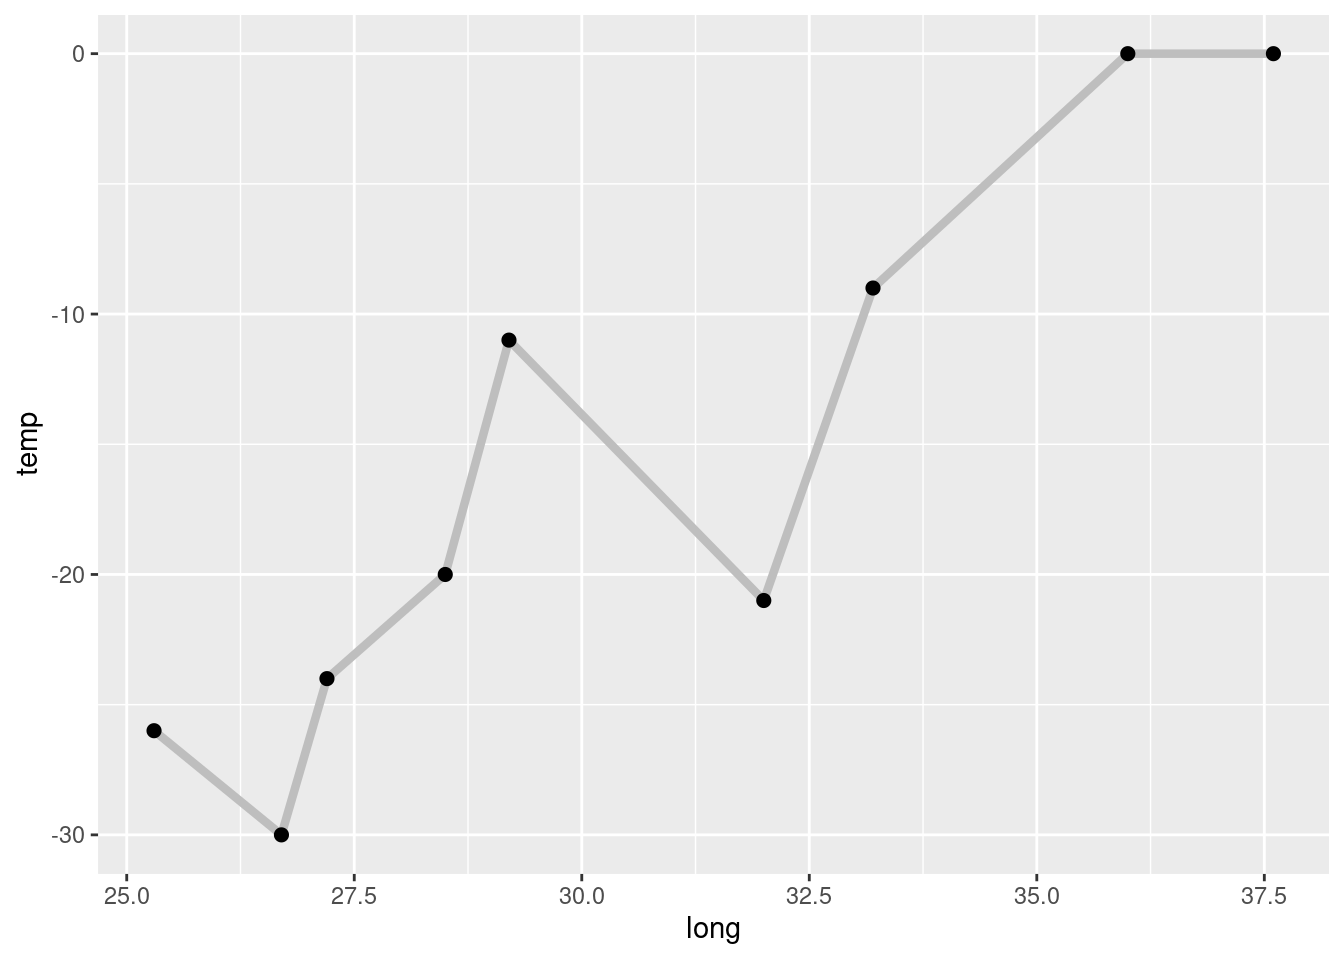
\includegraphics{lab1_files/figure-latex/unnamed-chunk-12-1.pdf}

\hypertarget{more-color}{%
\subsubsection{more color}\label{more-color}}

see \href{https://github.com/easystats/see}{see} for more color

\begin{Shaded}
\begin{Highlighting}[]
\FunctionTok{library}\NormalTok{(see)}
\CommentTok{\# https://github.com/easystats/see}

\NormalTok{mtcars }\SpecialCharTok{|}\ErrorTok{\textgreater{}} 
\FunctionTok{ggplot}\NormalTok{(}\FunctionTok{aes}\NormalTok{(}\AttributeTok{x =}\NormalTok{wt, }\AttributeTok{y =}\NormalTok{ mpg, }
           \AttributeTok{color =}\NormalTok{ gear }\SpecialCharTok{|}\ErrorTok{\textgreater{}} \FunctionTok{as\_factor}\NormalTok{())) }\SpecialCharTok{+}
  \FunctionTok{geom\_smooth}\NormalTok{(}\AttributeTok{method=}\StringTok{\textquotesingle{}lm\textquotesingle{}}\NormalTok{, }\AttributeTok{alpha =} \FloatTok{0.1}\NormalTok{, }\AttributeTok{size =} \DecValTok{0}\NormalTok{)}\SpecialCharTok{+}
  \FunctionTok{geom\_line}\NormalTok{(}\AttributeTok{stat=}\StringTok{"smooth"}\NormalTok{,}\AttributeTok{method =} \StringTok{"lm"}\NormalTok{, }\AttributeTok{size  =} \FloatTok{1.5}\NormalTok{, }\AttributeTok{alpha =} \FloatTok{0.5}\NormalTok{)}\SpecialCharTok{+}
  \FunctionTok{geom\_point}\NormalTok{(}\FunctionTok{aes}\NormalTok{(}\AttributeTok{size =}\NormalTok{ cyl }\SpecialCharTok{|}\ErrorTok{\textgreater{}} \FunctionTok{as.factor}\NormalTok{()))}\SpecialCharTok{+}
  \FunctionTok{ggtitle}\NormalTok{(}\StringTok{"4 D"}\NormalTok{, }\StringTok{"with statistics from basic attributes"}\NormalTok{)}\SpecialCharTok{+}
  \CommentTok{\# see::scale\_color\_material\_d()+}
\NormalTok{  see}\SpecialCharTok{::}\FunctionTok{scale\_color\_social}\NormalTok{()}\SpecialCharTok{+}
  \FunctionTok{theme\_minimal}\NormalTok{()}
\end{Highlighting}
\end{Shaded}

\begin{verbatim}
## Warning: Using size for a discrete variable is not advised.
\end{verbatim}

\begin{verbatim}
## `geom_smooth()` using formula 'y ~ x'
## `geom_smooth()` using formula 'y ~ x'
\end{verbatim}

\includegraphics{lab1_files/figure-latex/unnamed-chunk-13-1.pdf}

\hypertarget{real-data}{%
\subsection{real data}\label{real-data}}

\begin{Shaded}
\begin{Highlighting}[]
\NormalTok{bikes }\OtherTok{\textless{}{-}} \FunctionTok{read\_csv}\NormalTok{(}\StringTok{"\textasciitilde{}/r\_viz\_eu/data/Bike Sharing Demand.csv"}\NormalTok{)}
\end{Highlighting}
\end{Shaded}

\begin{verbatim}
## Rows: 10886 Columns: 12
## -- Column specification --------------------------------------------------------
## Delimiter: ","
## dbl  (11): season, holiday, workingday, weather, temp, atemp, humidity, wind...
## dttm  (1): datetime
## 
## i Use `spec()` to retrieve the full column specification for this data.
## i Specify the column types or set `show_col_types = FALSE` to quiet this message.
\end{verbatim}

\begin{Shaded}
\begin{Highlighting}[]
\NormalTok{bikes }\SpecialCharTok{|}\ErrorTok{\textgreater{}} \FunctionTok{head}\NormalTok{()}
\end{Highlighting}
\end{Shaded}

\begin{verbatim}
## # A tibble: 6 x 12
##   datetime            season holiday workingday weather  temp atemp humidity
##   <dttm>               <dbl>   <dbl>      <dbl>   <dbl> <dbl> <dbl>    <dbl>
## 1 2011-01-01 00:00:00      1       0          0       1  9.84  14.4       81
## 2 2011-01-01 01:00:00      1       0          0       1  9.02  13.6       80
## 3 2011-01-01 02:00:00      1       0          0       1  9.02  13.6       80
## 4 2011-01-01 03:00:00      1       0          0       1  9.84  14.4       75
## 5 2011-01-01 04:00:00      1       0          0       1  9.84  14.4       75
## 6 2011-01-01 05:00:00      1       0          0       2  9.84  12.9       75
## # ... with 4 more variables: windspeed <dbl>, casual <dbl>, registered <dbl>,
## #   count <dbl>
\end{verbatim}

\begin{Shaded}
\begin{Highlighting}[]
\NormalTok{bikes }\SpecialCharTok{|}\ErrorTok{\textgreater{}} 
  \FunctionTok{ggplot}\NormalTok{(}\FunctionTok{aes}\NormalTok{(}\AttributeTok{x =}\NormalTok{ holiday))}\SpecialCharTok{+}
  \FunctionTok{geom\_bar}\NormalTok{()}\SpecialCharTok{+}
  \FunctionTok{theme\_minimal}\NormalTok{()}
\end{Highlighting}
\end{Shaded}

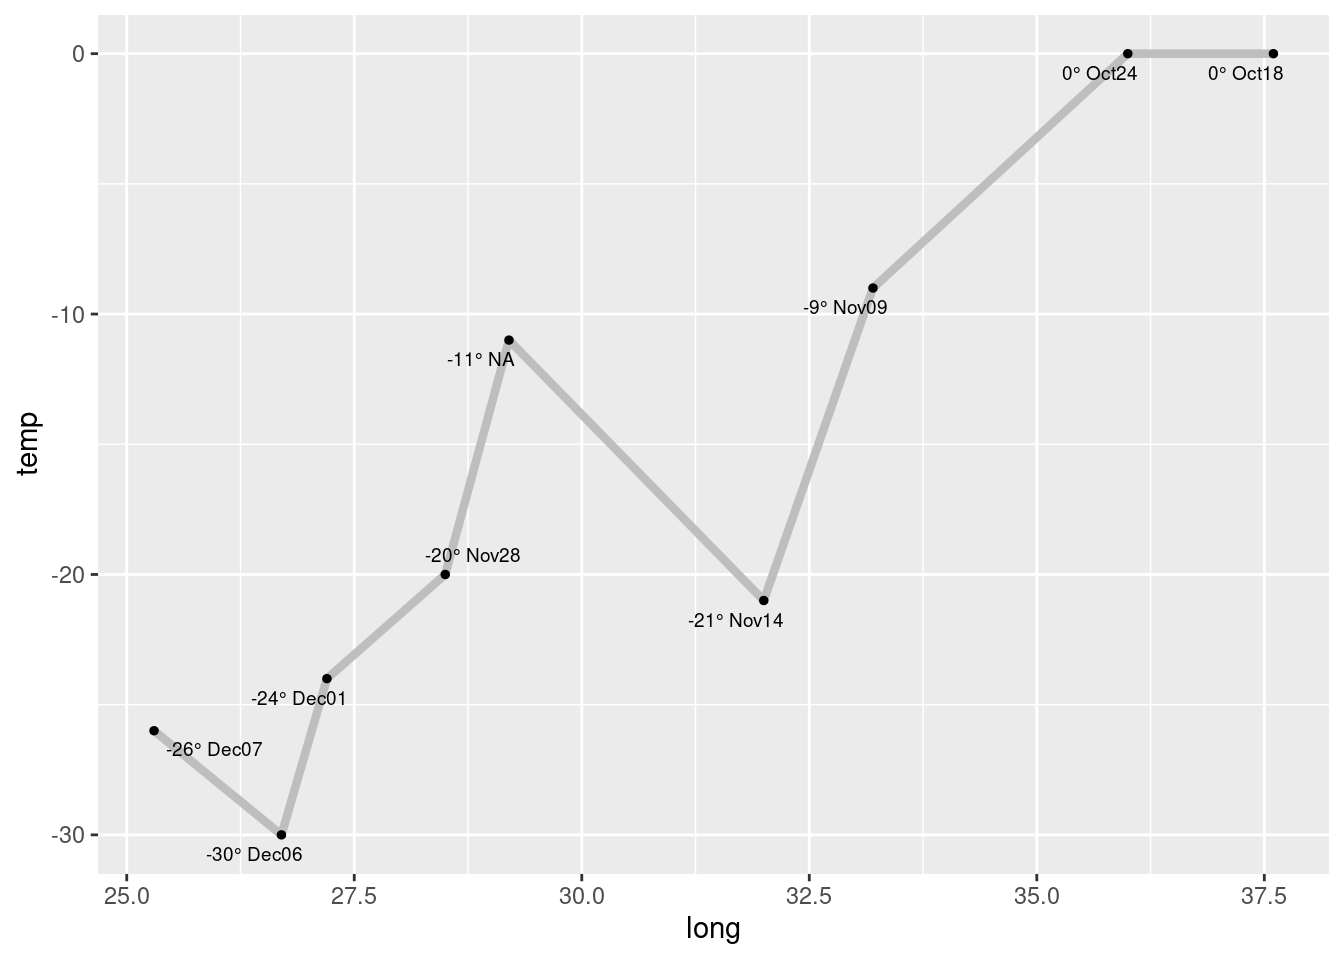
\includegraphics{lab1_files/figure-latex/unnamed-chunk-15-1.pdf}

You could try to turn count into percentage following the tutorial

\href{https://sebastiansauer.github.io/percentage_plot_ggplot2_V2/}{How
to plot a `percentage plot' with ggplot2 -- Sebastian Sauer Stats Blog}

\begin{Shaded}
\begin{Highlighting}[]
\CommentTok{\# bikes |\textgreater{} }
\end{Highlighting}
\end{Shaded}

\begin{Shaded}
\begin{Highlighting}[]
\NormalTok{bikes }\SpecialCharTok{|}\ErrorTok{\textgreater{}} 
  \FunctionTok{group\_by}\NormalTok{(holiday) }\SpecialCharTok{|}\ErrorTok{\textgreater{}} 
  \FunctionTok{summarise}\NormalTok{(}\AttributeTok{count =} \FunctionTok{sum}\NormalTok{(count)) }\SpecialCharTok{|}\ErrorTok{\textgreater{}} 
    \FunctionTok{ggplot}\NormalTok{(}\FunctionTok{aes}\NormalTok{(}\AttributeTok{x =}\NormalTok{ holiday, }\AttributeTok{y =}\NormalTok{ count))}\SpecialCharTok{+}
    \FunctionTok{geom\_bar}\NormalTok{(}\AttributeTok{stat =} \StringTok{"identity"}\NormalTok{)}\SpecialCharTok{+}
    \FunctionTok{theme\_minimal}\NormalTok{()}
\end{Highlighting}
\end{Shaded}

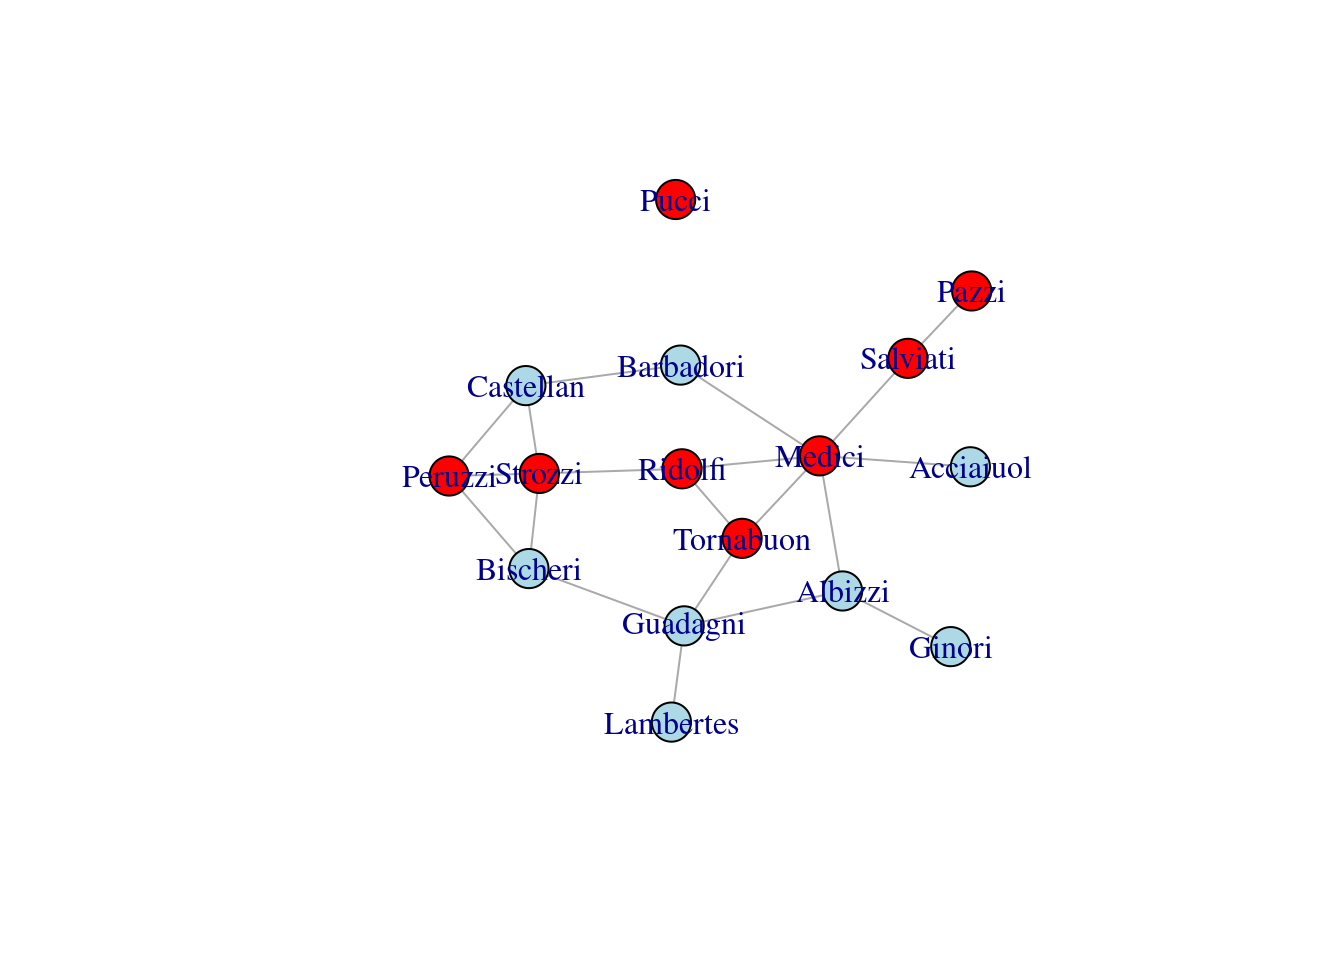
\includegraphics{lab1_files/figure-latex/unnamed-chunk-17-1.pdf}

\begin{Shaded}
\begin{Highlighting}[]
\NormalTok{bikes }\SpecialCharTok{|}\ErrorTok{\textgreater{}} 
  \FunctionTok{mutate}\NormalTok{(}\AttributeTok{holiday =}\NormalTok{ holiday }\SpecialCharTok{|}\ErrorTok{\textgreater{}} \FunctionTok{as.logical}\NormalTok{()) }\SpecialCharTok{|}\ErrorTok{\textgreater{}} 
    \FunctionTok{ggplot}\NormalTok{(}\FunctionTok{aes}\NormalTok{(}\AttributeTok{x =}\NormalTok{ holiday, }\AttributeTok{y =}\NormalTok{ count))}\SpecialCharTok{+}
    \FunctionTok{geom\_boxplot}\NormalTok{()}\SpecialCharTok{+}
    \FunctionTok{theme\_minimal}\NormalTok{()}
\end{Highlighting}
\end{Shaded}

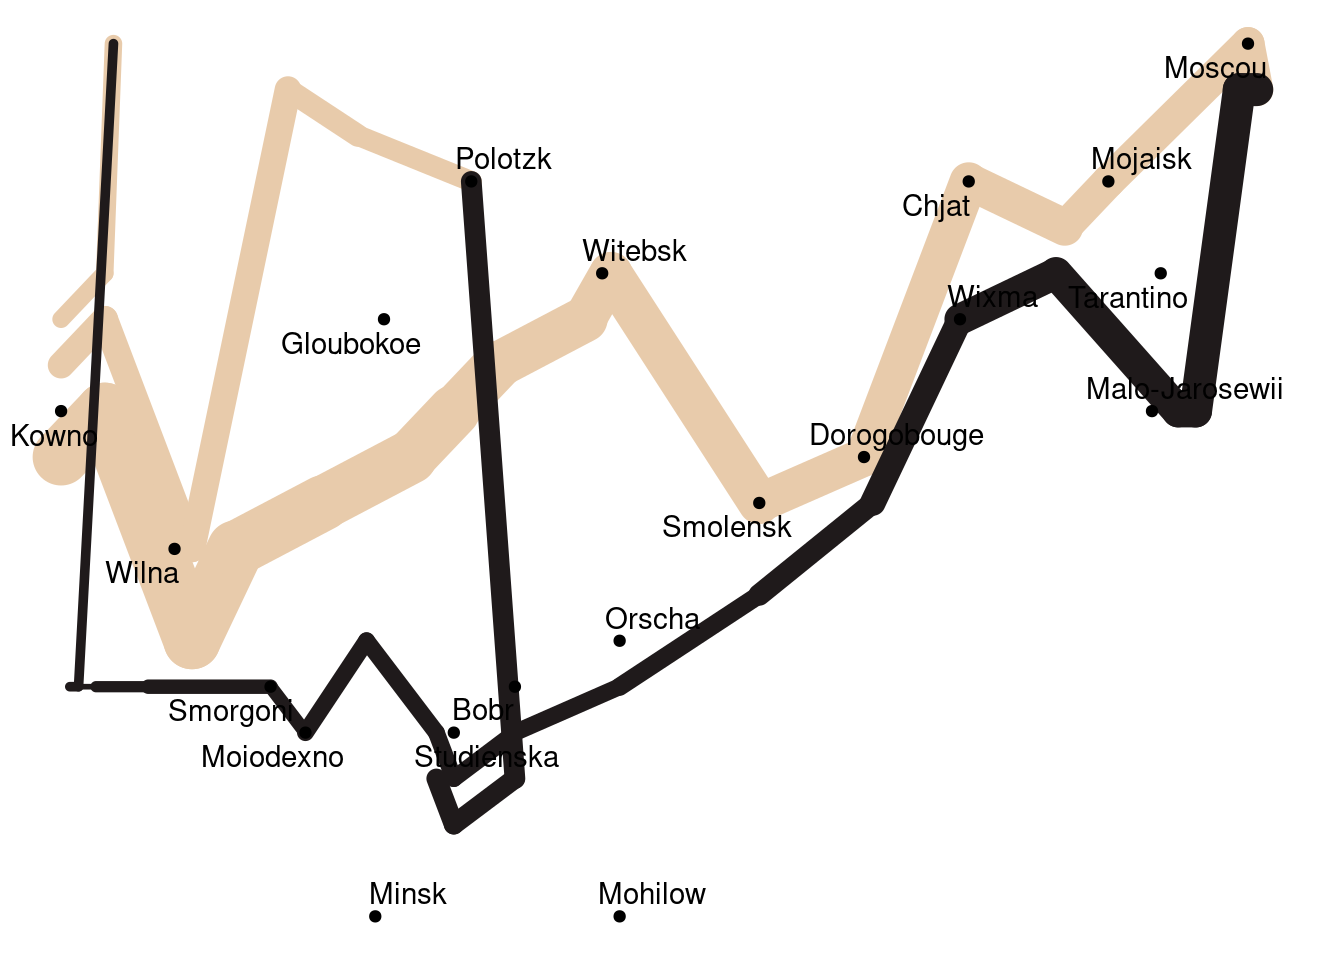
\includegraphics{lab1_files/figure-latex/unnamed-chunk-18-1.pdf}

Why do we have almost the same median for holidays and non holidays?

\begin{Shaded}
\begin{Highlighting}[]
\NormalTok{bikes }\SpecialCharTok{|}\ErrorTok{\textgreater{}} 
  \FunctionTok{mutate}\NormalTok{(}\AttributeTok{holiday =}\NormalTok{ holiday }\SpecialCharTok{|}\ErrorTok{\textgreater{}} \FunctionTok{as.logical}\NormalTok{()) }\SpecialCharTok{|}\ErrorTok{\textgreater{}} 
    \FunctionTok{ggplot}\NormalTok{(}\FunctionTok{aes}\NormalTok{(}\AttributeTok{x =}\NormalTok{ holiday, }\AttributeTok{y =}\NormalTok{ count))}\SpecialCharTok{+}
    \FunctionTok{geom\_boxplot}\NormalTok{()}\SpecialCharTok{+}
    \FunctionTok{geom\_jitter}\NormalTok{(}\AttributeTok{alpha =} \FloatTok{0.1}\NormalTok{)}\SpecialCharTok{+}
    \FunctionTok{theme\_minimal}\NormalTok{()}
\end{Highlighting}
\end{Shaded}

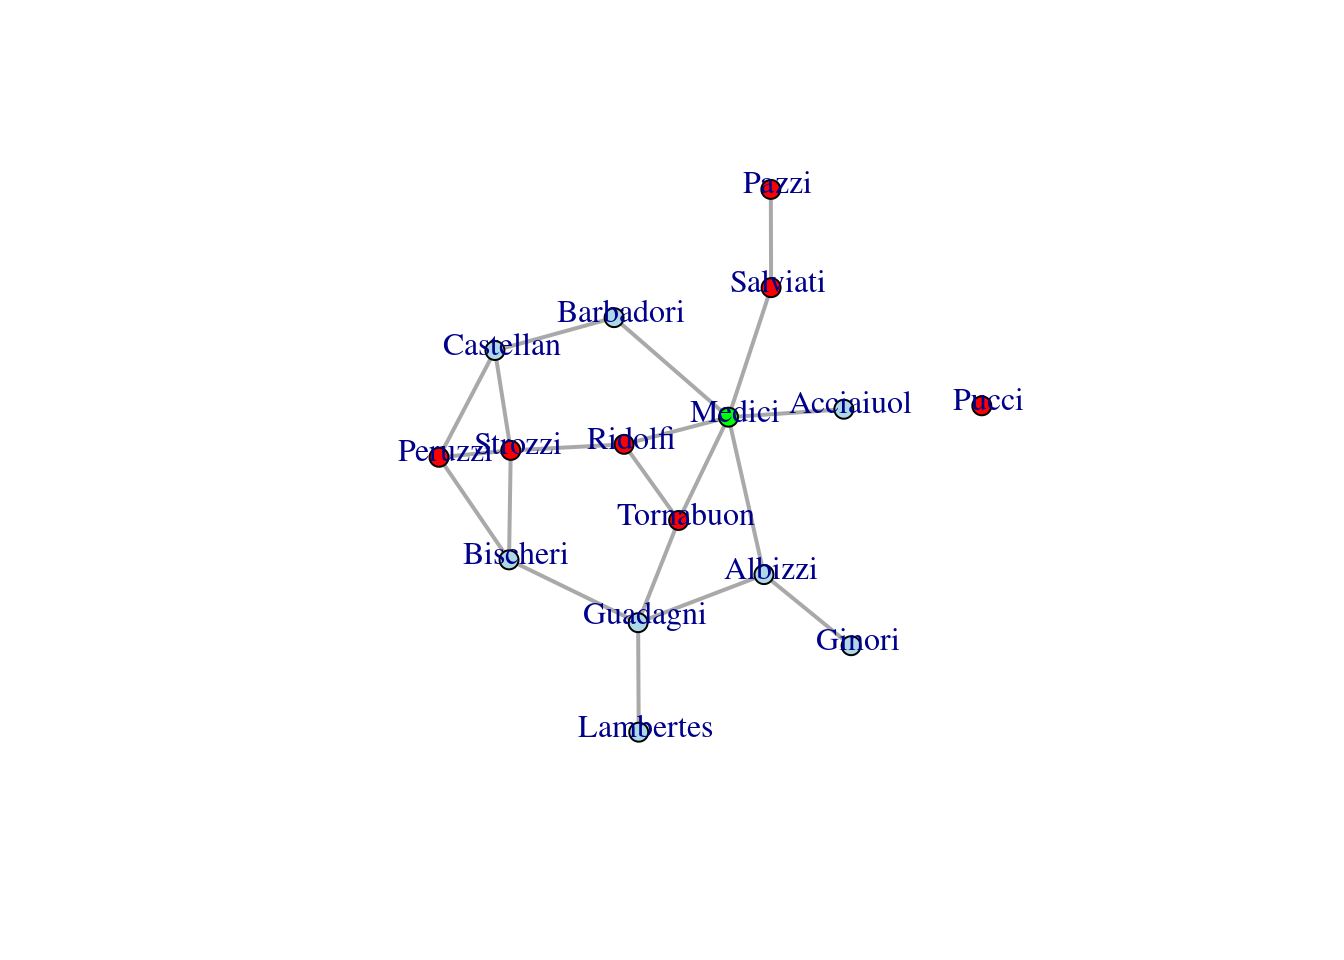
\includegraphics{lab1_files/figure-latex/unnamed-chunk-19-1.pdf}

\begin{Shaded}
\begin{Highlighting}[]
\NormalTok{bikes }\SpecialCharTok{|}\ErrorTok{\textgreater{}} 
  \FunctionTok{mutate}\NormalTok{(}\AttributeTok{holiday =}\NormalTok{ holiday }\SpecialCharTok{|}\ErrorTok{\textgreater{}} \FunctionTok{as.logical}\NormalTok{()) }\SpecialCharTok{|}\ErrorTok{\textgreater{}} 
    \FunctionTok{ggplot}\NormalTok{(}\FunctionTok{aes}\NormalTok{(}\AttributeTok{x =}\NormalTok{ holiday, }\AttributeTok{y =}\NormalTok{ count))}\SpecialCharTok{+}
    \FunctionTok{geom\_violin}\NormalTok{(}\AttributeTok{draw\_quantiles =} \FunctionTok{c}\NormalTok{(}\FloatTok{0.25}\NormalTok{, }\FloatTok{0.5}\NormalTok{, }\FloatTok{0.75}\NormalTok{), }\AttributeTok{trim =} \ConstantTok{FALSE}\NormalTok{)}\SpecialCharTok{+}
    \FunctionTok{geom\_jitter}\NormalTok{(}\AttributeTok{alpha =} \FloatTok{0.1}\NormalTok{)}\SpecialCharTok{+}
    \FunctionTok{theme\_minimal}\NormalTok{()}
\end{Highlighting}
\end{Shaded}

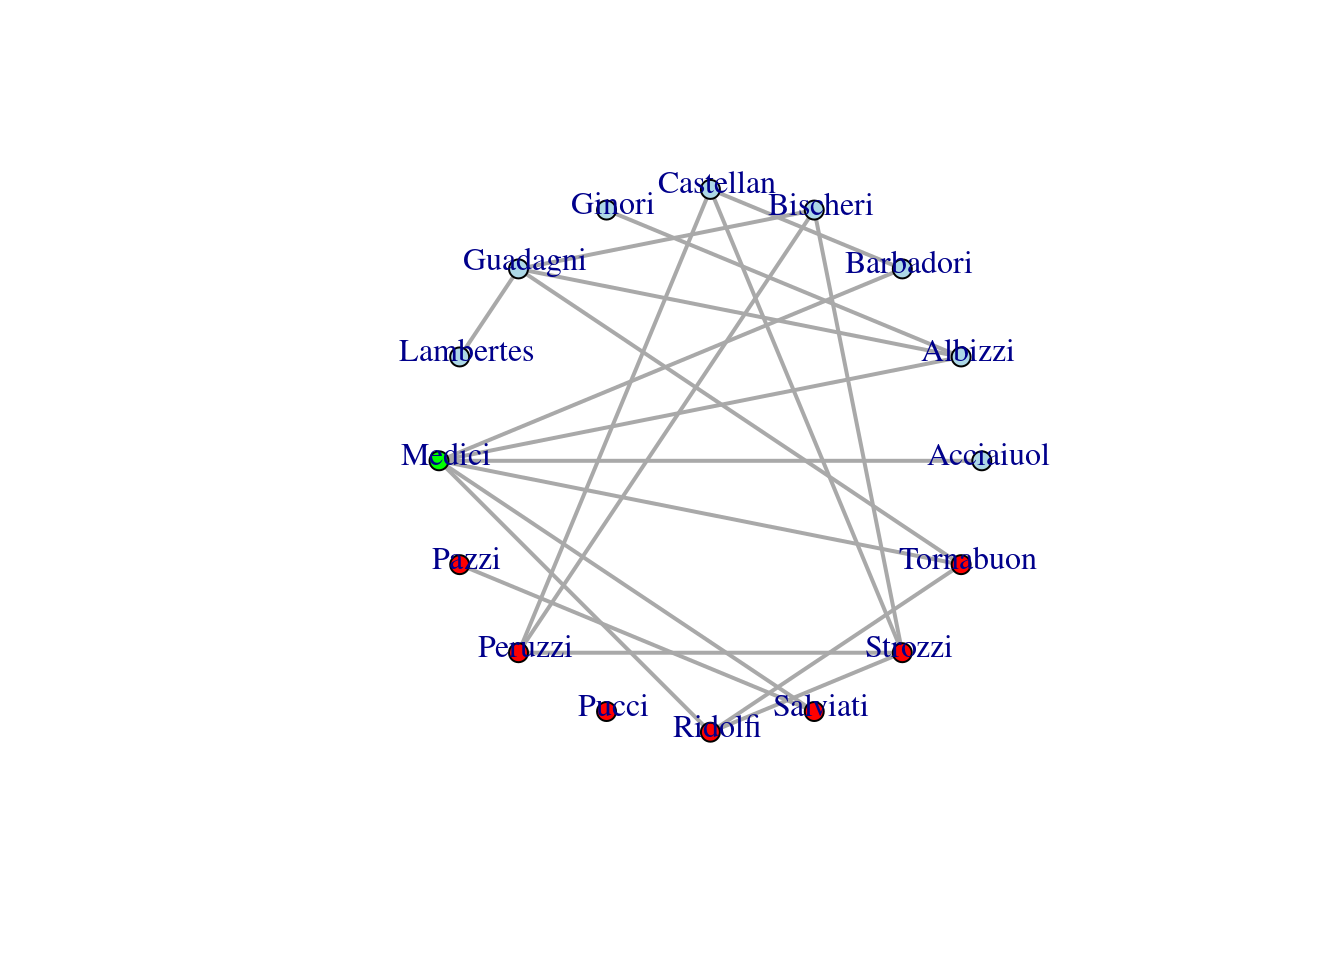
\includegraphics{lab1_files/figure-latex/unnamed-chunk-20-1.pdf}

\begin{Shaded}
\begin{Highlighting}[]
\FunctionTok{library}\NormalTok{(ggpubr)}

\NormalTok{bikes }\SpecialCharTok{|}\ErrorTok{\textgreater{}} 
  \FunctionTok{ggboxplot}\NormalTok{(}\AttributeTok{x =} \StringTok{"holiday"}\NormalTok{, }\AttributeTok{y =} \StringTok{"count"}\NormalTok{,}
            \AttributeTok{color =} \StringTok{"holiday"}\NormalTok{, }\AttributeTok{palette =}\FunctionTok{c}\NormalTok{(}\StringTok{"\#00AFBB"}\NormalTok{, }\StringTok{"\#E7B800"}\NormalTok{)) }\OtherTok{{-}\textgreater{}}\NormalTok{ p}
\NormalTok{p}
\end{Highlighting}
\end{Shaded}

\includegraphics{lab1_files/figure-latex/unnamed-chunk-21-1.pdf}

\begin{Shaded}
\begin{Highlighting}[]
 \CommentTok{\# Add p{-}values comparing groups}
 \CommentTok{\# Specify the comparisons you want}
\NormalTok{my\_comparisons }\OtherTok{\textless{}{-}} \FunctionTok{list}\NormalTok{( }\FunctionTok{c}\NormalTok{(}\DecValTok{0}\NormalTok{, }\DecValTok{1}\NormalTok{))}
\NormalTok{p }\SpecialCharTok{+} 
  \FunctionTok{stat\_compare\_means}\NormalTok{(}\AttributeTok{comparisons =}\NormalTok{ my\_comparisons)}\SpecialCharTok{+} 
  \CommentTok{\# Add pairwise comparisons p{-}value}
  \FunctionTok{stat\_compare\_means}\NormalTok{(}\AttributeTok{label.y =} \DecValTok{50}\NormalTok{)                   }\CommentTok{\# Add global p{-}value}
\end{Highlighting}
\end{Shaded}

\includegraphics{lab1_files/figure-latex/unnamed-chunk-21-2.pdf}

\begin{Shaded}
\begin{Highlighting}[]
\NormalTok{bikes }\SpecialCharTok{|}\ErrorTok{\textgreater{}} 
  \FunctionTok{ggboxplot}\NormalTok{(}\AttributeTok{x =} \StringTok{"season"}\NormalTok{, }\AttributeTok{y =} \StringTok{"count"}\NormalTok{,}
            \AttributeTok{color =} \StringTok{"season"}\NormalTok{, }\AttributeTok{palette =}\StringTok{"npg"}\NormalTok{) }\OtherTok{{-}\textgreater{}}\NormalTok{ p2}
\NormalTok{p2}
\end{Highlighting}
\end{Shaded}

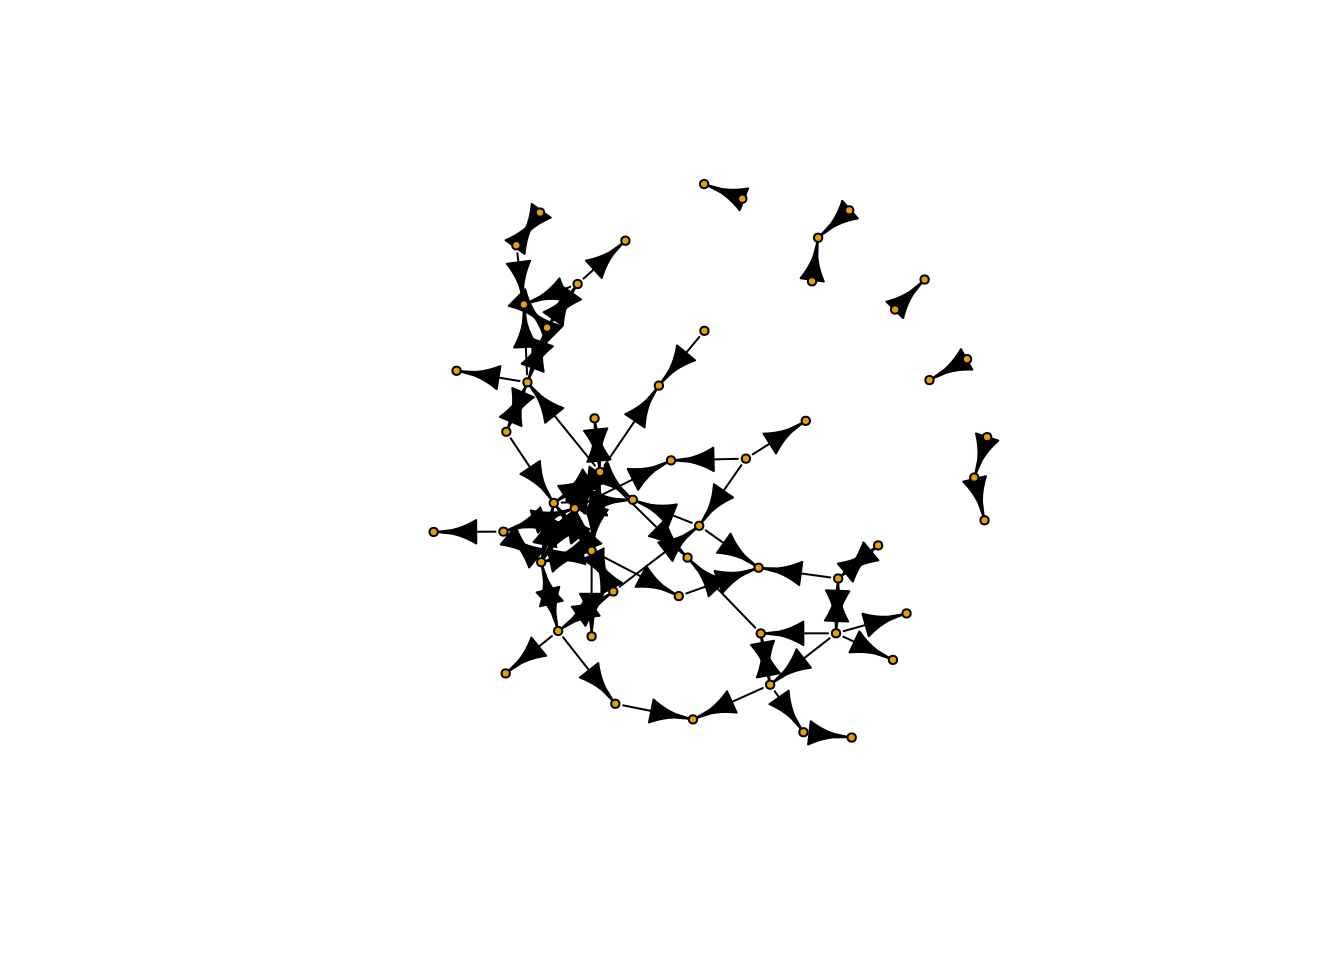
\includegraphics{lab1_files/figure-latex/unnamed-chunk-22-1.pdf}

\begin{Shaded}
\begin{Highlighting}[]
 \CommentTok{\# Add p{-}values comparing groups}
 \CommentTok{\# Specify the comparisons you want}
\NormalTok{my\_comparisons }\OtherTok{\textless{}{-}} \FunctionTok{combn}\NormalTok{(}\FunctionTok{c}\NormalTok{(}\DecValTok{1}\NormalTok{, }\DecValTok{2}\NormalTok{, }\DecValTok{3}\NormalTok{, }\DecValTok{4}\NormalTok{), }\AttributeTok{m =} \DecValTok{2}\NormalTok{, }\AttributeTok{simplify =}\NormalTok{ F)}
\NormalTok{p2 }\SpecialCharTok{+} 
  \FunctionTok{stat\_compare\_means}\NormalTok{(}\AttributeTok{comparisons =}\NormalTok{ my\_comparisons)}\SpecialCharTok{+} 
  \CommentTok{\# Add pairwise comparisons p{-}value}
  \FunctionTok{stat\_compare\_means}\NormalTok{(}\AttributeTok{label.y =} \DecValTok{1600}\NormalTok{)}
\end{Highlighting}
\end{Shaded}

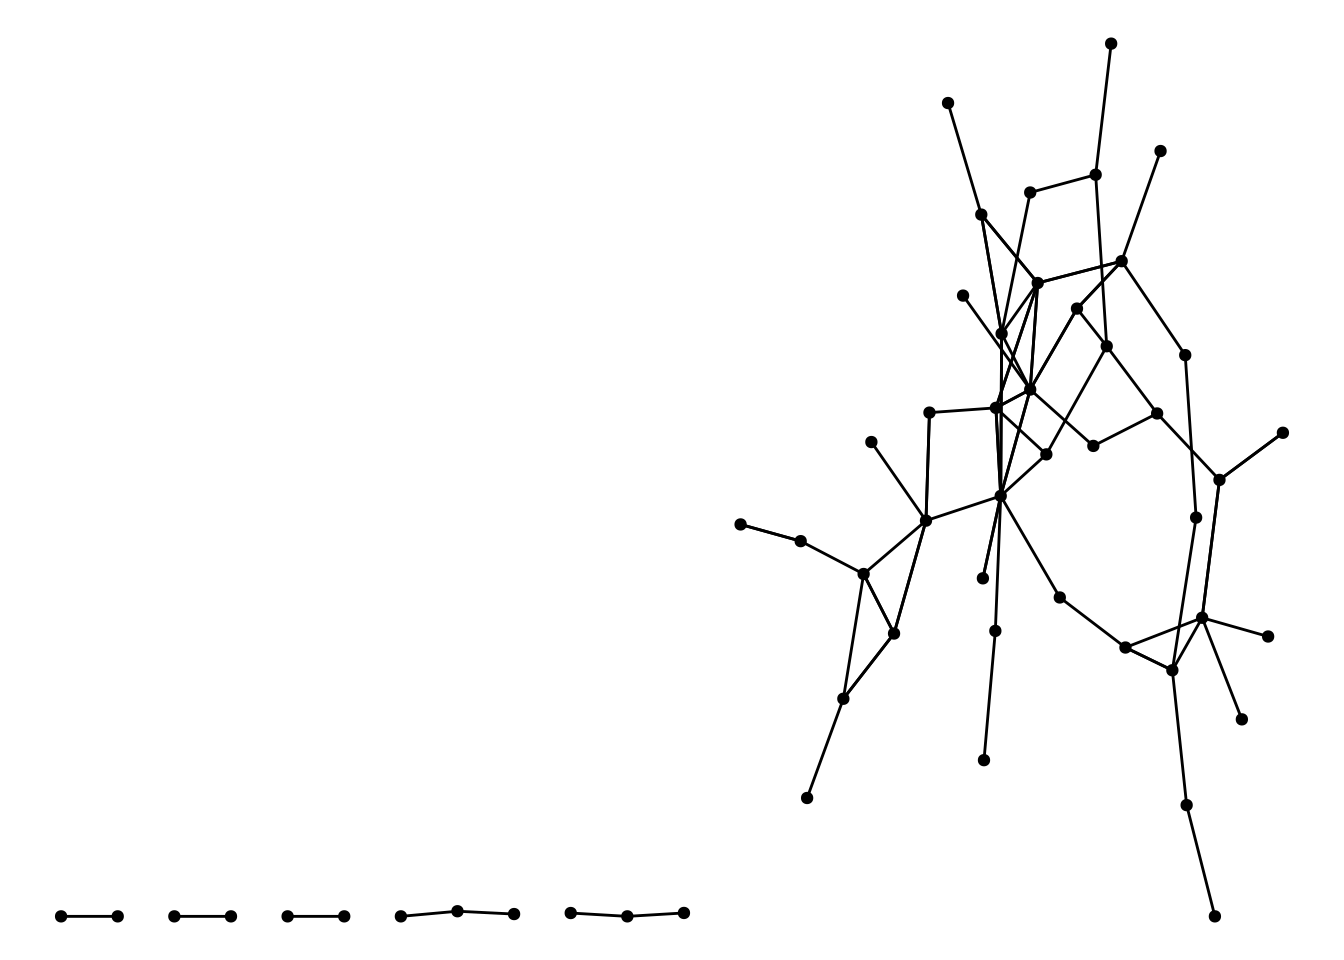
\includegraphics{lab1_files/figure-latex/unnamed-chunk-22-2.pdf}

\hypertarget{manipulations-and-data-quality}{%
\subsubsection{manipulations and data
quality}\label{manipulations-and-data-quality}}

\begin{Shaded}
\begin{Highlighting}[]
\NormalTok{bikes }\SpecialCharTok{|}\ErrorTok{\textgreater{}} 
  \FunctionTok{ggplot}\NormalTok{(}\FunctionTok{aes}\NormalTok{(}\AttributeTok{x =}\NormalTok{ atemp, }\AttributeTok{y =}\NormalTok{ count))}\SpecialCharTok{+}
  \FunctionTok{geom\_point}\NormalTok{()}\SpecialCharTok{+}
  \FunctionTok{geom\_smooth}\NormalTok{(}\AttributeTok{method =} \StringTok{"lm"}\NormalTok{)}\SpecialCharTok{+}
  \FunctionTok{theme\_minimal}\NormalTok{()}
\end{Highlighting}
\end{Shaded}

\begin{verbatim}
## `geom_smooth()` using formula 'y ~ x'
\end{verbatim}

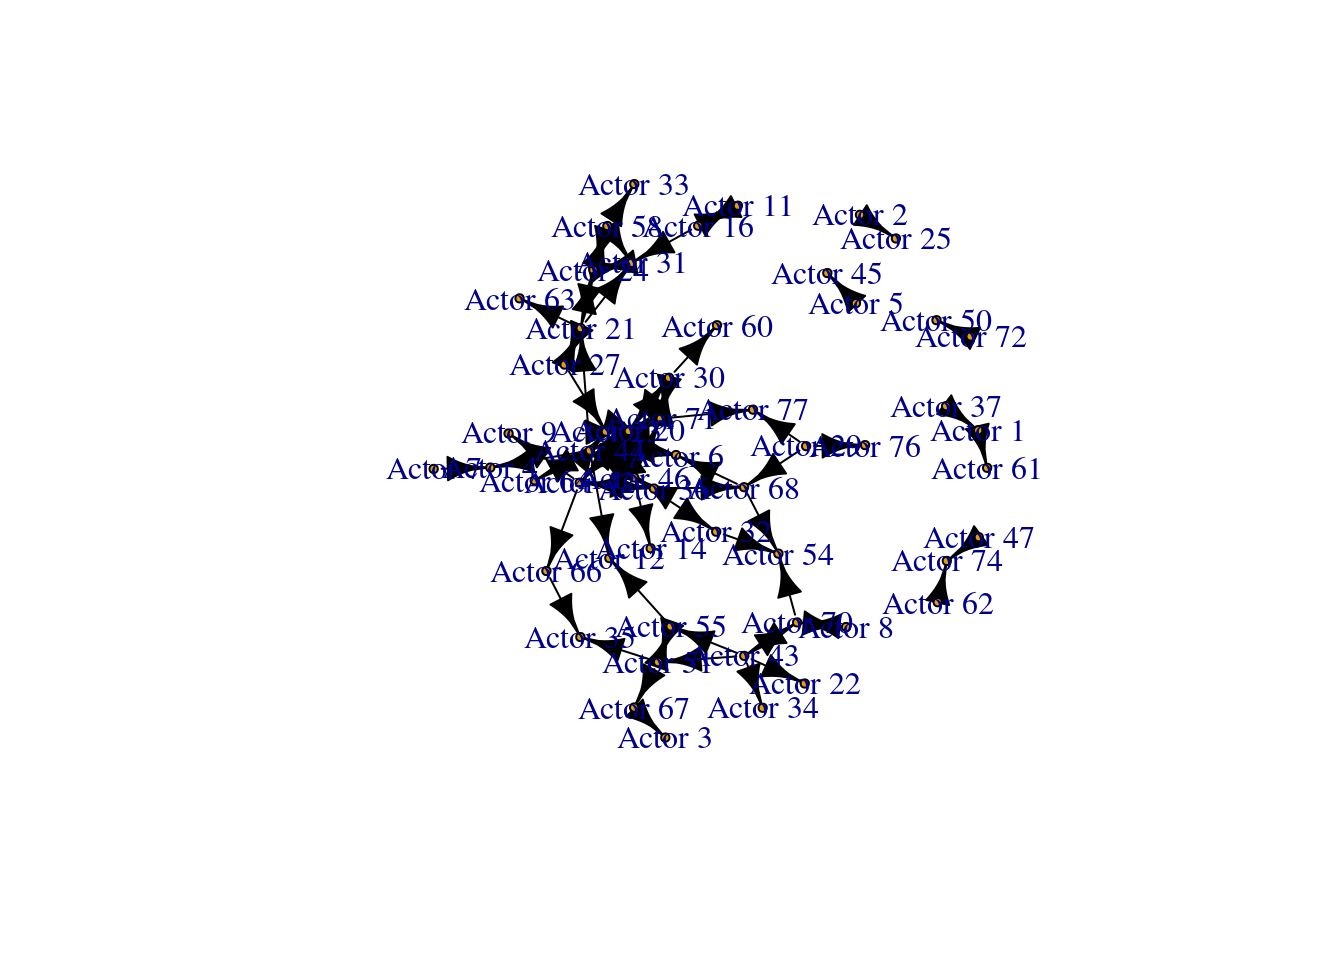
\includegraphics{lab1_files/figure-latex/unnamed-chunk-23-1.pdf}

\begin{Shaded}
\begin{Highlighting}[]
\NormalTok{bikes }\SpecialCharTok{|}\ErrorTok{\textgreater{}} 
  \FunctionTok{ggplot}\NormalTok{(}\FunctionTok{aes}\NormalTok{(}\AttributeTok{x =}\NormalTok{ atemp, }\AttributeTok{y =}\NormalTok{ count))}\SpecialCharTok{+}
  \FunctionTok{geom\_point}\NormalTok{()}\SpecialCharTok{+}
  \FunctionTok{geom\_smooth}\NormalTok{(}\AttributeTok{method =} \StringTok{"lm"}\NormalTok{)}\SpecialCharTok{+}
  \FunctionTok{theme\_minimal}\NormalTok{()}\SpecialCharTok{+}
    \FunctionTok{scale\_y\_log10}\NormalTok{()}
\end{Highlighting}
\end{Shaded}

\begin{verbatim}
## `geom_smooth()` using formula 'y ~ x'
\end{verbatim}

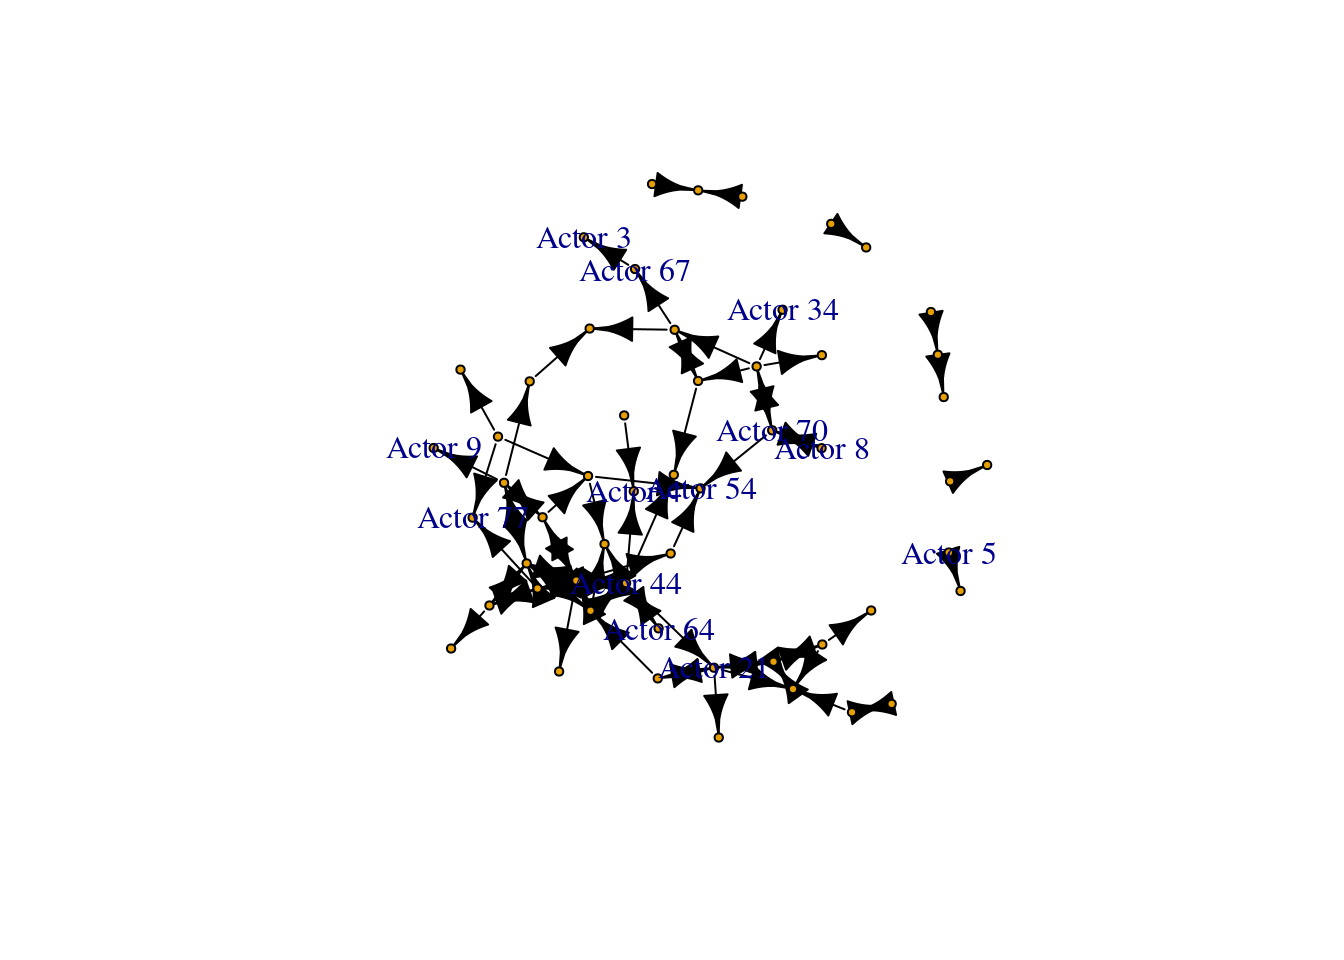
\includegraphics{lab1_files/figure-latex/unnamed-chunk-24-1.pdf}

\begin{Shaded}
\begin{Highlighting}[]
\NormalTok{bikes }\SpecialCharTok{|}\ErrorTok{\textgreater{}} 
  \FunctionTok{filter}\NormalTok{(atemp}\SpecialCharTok{\textgreater{}=}\DecValTok{30} \SpecialCharTok{\&}\NormalTok{ atemp }\SpecialCharTok{\textless{}=}\DecValTok{45}\NormalTok{) }\SpecialCharTok{|}\ErrorTok{\textgreater{}} 
  \FunctionTok{ggplot}\NormalTok{(}\FunctionTok{aes}\NormalTok{(}\AttributeTok{x =}\NormalTok{ atemp, }\AttributeTok{y =}\NormalTok{ count))}\SpecialCharTok{+}
  \FunctionTok{geom\_point}\NormalTok{()}\SpecialCharTok{+}
  \FunctionTok{geom\_smooth}\NormalTok{(}\AttributeTok{method =} \StringTok{"lm"}\NormalTok{)}\SpecialCharTok{+}
    \FunctionTok{scale\_y\_log10}\NormalTok{()}\SpecialCharTok{+}
  \FunctionTok{xlim}\NormalTok{(}\DecValTok{30}\NormalTok{, }\DecValTok{45}\NormalTok{)}\SpecialCharTok{+}
  \FunctionTok{theme\_minimal}\NormalTok{()}
\end{Highlighting}
\end{Shaded}

\begin{verbatim}
## `geom_smooth()` using formula 'y ~ x'
\end{verbatim}

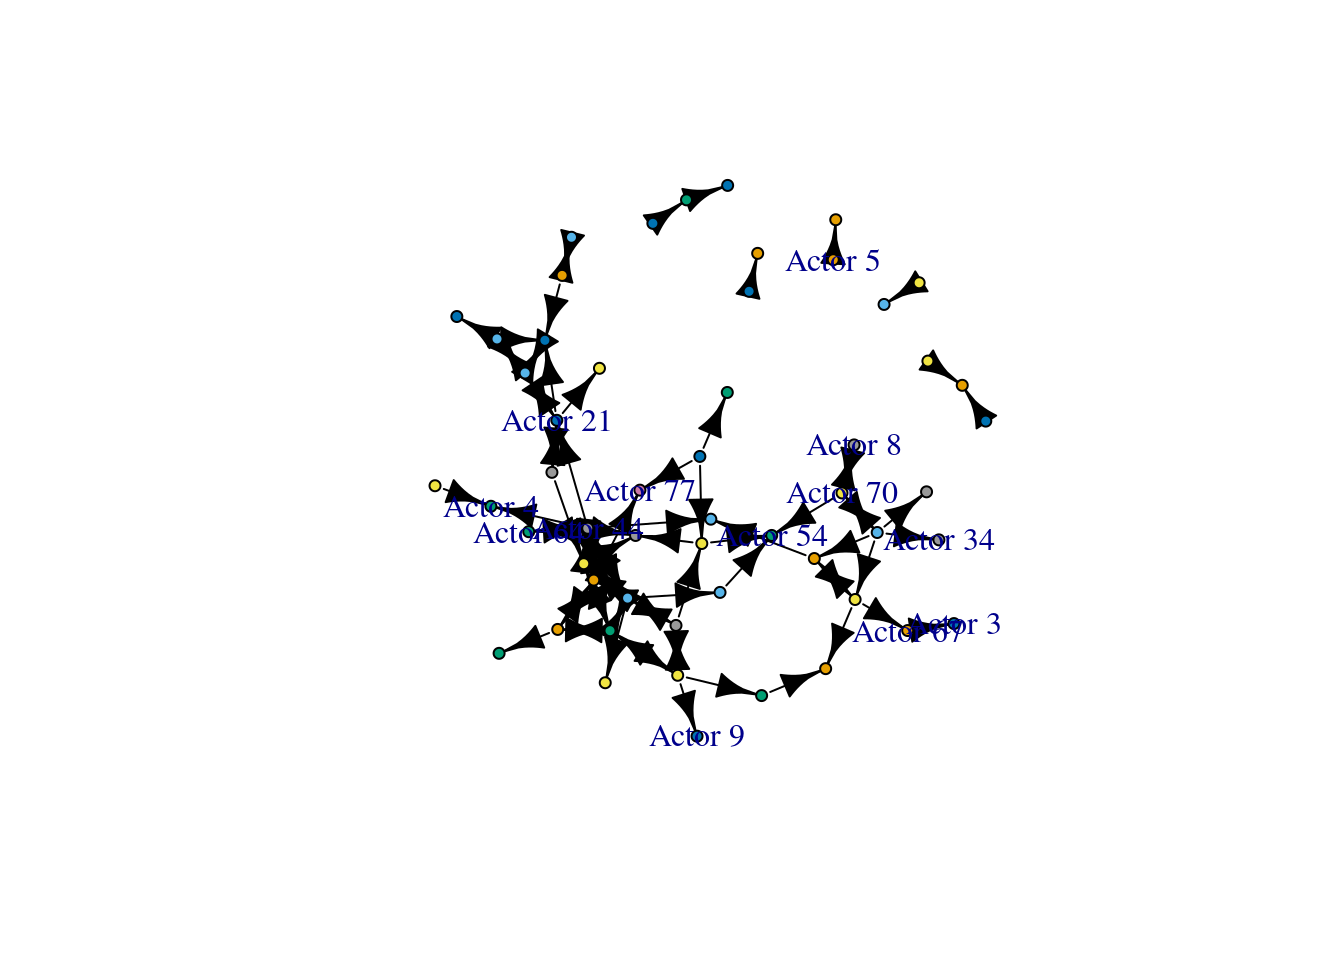
\includegraphics{lab1_files/figure-latex/unnamed-chunk-25-1.pdf}

\hypertarget{kind-of-a-solution}{%
\subsubsection{kind of a solution}\label{kind-of-a-solution}}

\begin{Shaded}
\begin{Highlighting}[]
\NormalTok{bikes }\SpecialCharTok{|}\ErrorTok{\textgreater{}} 
  \FunctionTok{ggplot}\NormalTok{(}\FunctionTok{aes}\NormalTok{(}\AttributeTok{x =}\NormalTok{ atemp, }\AttributeTok{y =}\NormalTok{ count))}\SpecialCharTok{+}
  \FunctionTok{geom\_jitter}\NormalTok{(}\AttributeTok{width =} \FloatTok{0.2}\NormalTok{, }\AttributeTok{height =} \FloatTok{0.2}\NormalTok{, }\AttributeTok{alpha =} \FloatTok{0.4}\NormalTok{)}\SpecialCharTok{+}
  \FunctionTok{geom\_smooth}\NormalTok{(}\AttributeTok{method =} \StringTok{"lm"}\NormalTok{)}\SpecialCharTok{+}
  \FunctionTok{scale\_y\_log10}\NormalTok{()}\SpecialCharTok{+}
  \FunctionTok{theme\_minimal}\NormalTok{()}
\end{Highlighting}
\end{Shaded}

\begin{verbatim}
## `geom_smooth()` using formula 'y ~ x'
\end{verbatim}

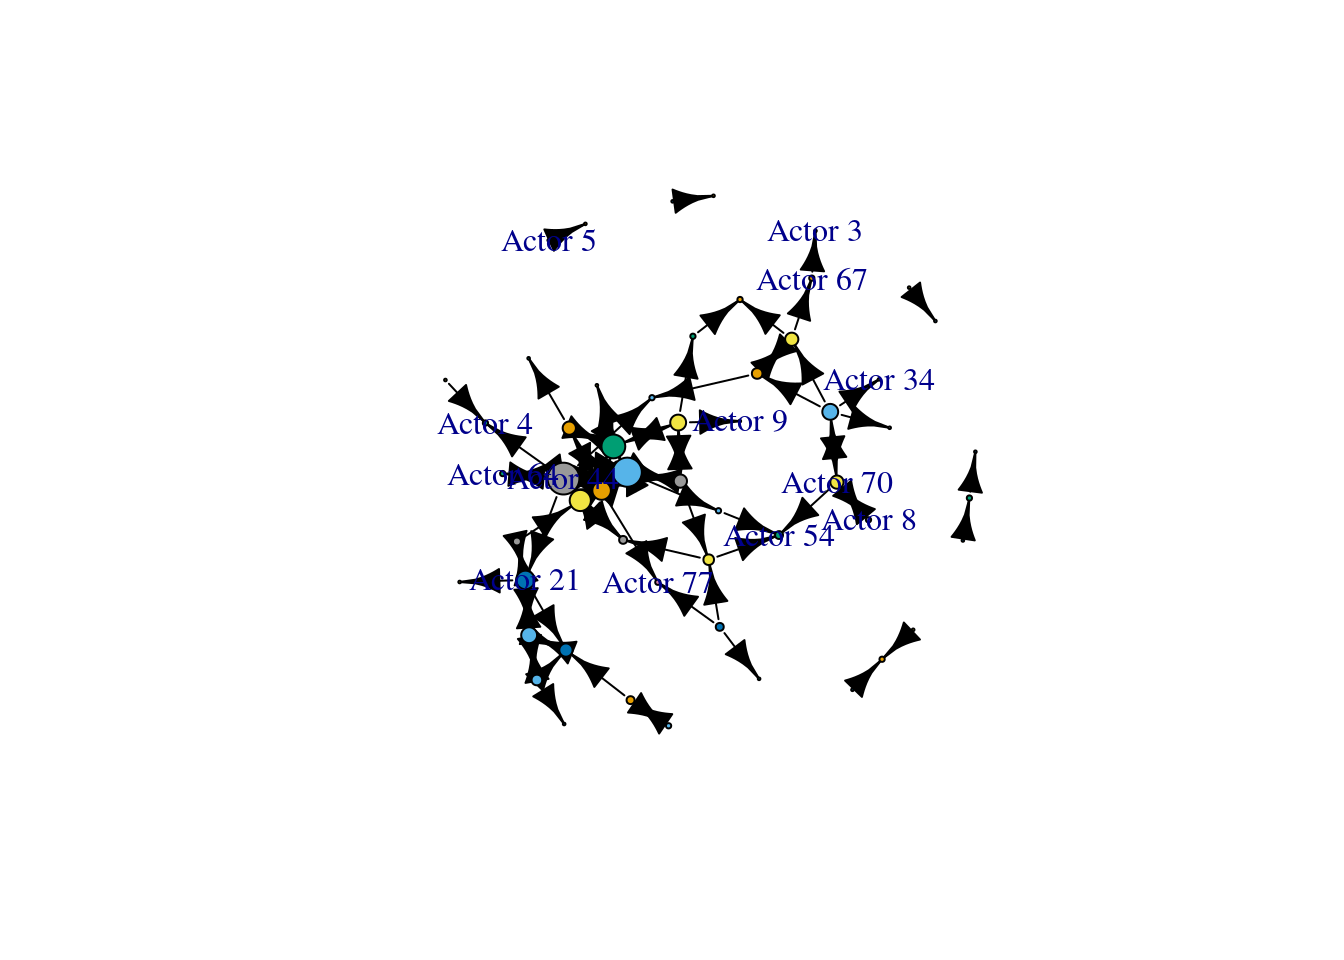
\includegraphics{lab1_files/figure-latex/unnamed-chunk-26-1.pdf}

\begin{Shaded}
\begin{Highlighting}[]
\NormalTok{bikes }\SpecialCharTok{|}\ErrorTok{\textgreater{}} 
  \FunctionTok{ggplot}\NormalTok{(}\FunctionTok{aes}\NormalTok{(}\AttributeTok{x =}\NormalTok{ atemp, }\AttributeTok{y =}\NormalTok{ count))}\SpecialCharTok{+}
  \FunctionTok{geom\_jitter}\NormalTok{(}\AttributeTok{width =} \FloatTok{0.2}\NormalTok{, }\AttributeTok{height =} \FloatTok{0.2}\NormalTok{, }\AttributeTok{alpha =} \FloatTok{0.4}\NormalTok{)}\SpecialCharTok{+}
  \FunctionTok{geom\_smooth}\NormalTok{(}\AttributeTok{method =} \StringTok{"lm"}\NormalTok{)}\SpecialCharTok{+}
  \FunctionTok{scale\_y\_log10}\NormalTok{()}\SpecialCharTok{+}
  \FunctionTok{theme\_minimal}\NormalTok{()}
\end{Highlighting}
\end{Shaded}

\begin{verbatim}
## `geom_smooth()` using formula 'y ~ x'
\end{verbatim}

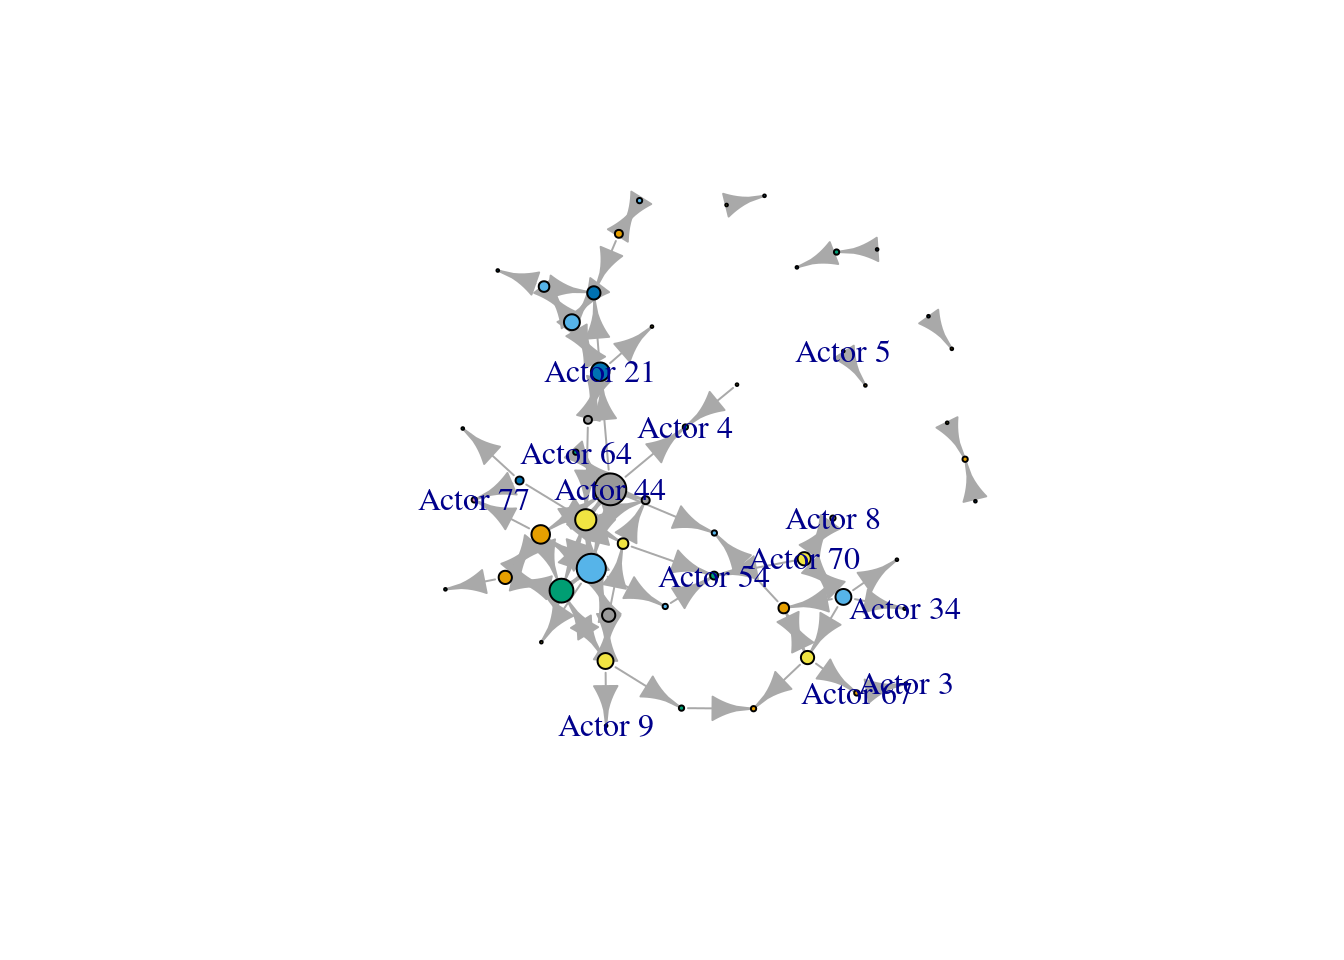
\includegraphics{lab1_files/figure-latex/unnamed-chunk-27-1.pdf}

\hypertarget{diamonds}{%
\subsubsection{diamonds}\label{diamonds}}

\begin{Shaded}
\begin{Highlighting}[]
\NormalTok{?diamonds}

\NormalTok{diamonds }\SpecialCharTok{|}\ErrorTok{\textgreater{}} 
  \FunctionTok{head}\NormalTok{()}
\end{Highlighting}
\end{Shaded}

\begin{verbatim}
## # A tibble: 6 x 10
##   carat cut       color clarity depth table price     x     y     z
##   <dbl> <ord>     <ord> <ord>   <dbl> <dbl> <int> <dbl> <dbl> <dbl>
## 1  0.23 Ideal     E     SI2      61.5    55   326  3.95  3.98  2.43
## 2  0.21 Premium   E     SI1      59.8    61   326  3.89  3.84  2.31
## 3  0.23 Good      E     VS1      56.9    65   327  4.05  4.07  2.31
## 4  0.29 Premium   I     VS2      62.4    58   334  4.2   4.23  2.63
## 5  0.31 Good      J     SI2      63.3    58   335  4.34  4.35  2.75
## 6  0.24 Very Good J     VVS2     62.8    57   336  3.94  3.96  2.48
\end{verbatim}

\begin{Shaded}
\begin{Highlighting}[]
\NormalTok{diamonds }\SpecialCharTok{|}\ErrorTok{\textgreater{}} 
  \FunctionTok{ggplot}\NormalTok{(}\FunctionTok{aes}\NormalTok{(}\AttributeTok{x =}\NormalTok{ carat, }\AttributeTok{y =}\NormalTok{ price))}\SpecialCharTok{+}
  \FunctionTok{geom\_point}\NormalTok{()}\SpecialCharTok{+}
  \FunctionTok{theme\_minimal}\NormalTok{()}
\end{Highlighting}
\end{Shaded}

\includegraphics{lab1_files/figure-latex/unnamed-chunk-29-1.pdf}

\begin{Shaded}
\begin{Highlighting}[]
\NormalTok{diamonds }\SpecialCharTok{|}\ErrorTok{\textgreater{}} 
  \FunctionTok{ggplot}\NormalTok{(}\FunctionTok{aes}\NormalTok{(}\AttributeTok{x =}\NormalTok{ carat, }\AttributeTok{y =}\NormalTok{ price))}\SpecialCharTok{+}
  \FunctionTok{geom\_point}\NormalTok{()}\SpecialCharTok{+}
  \FunctionTok{scale\_x\_log10}\NormalTok{()}\SpecialCharTok{+}
  \FunctionTok{scale\_y\_log10}\NormalTok{()}\SpecialCharTok{+}
  \FunctionTok{theme\_minimal}\NormalTok{()}
\end{Highlighting}
\end{Shaded}

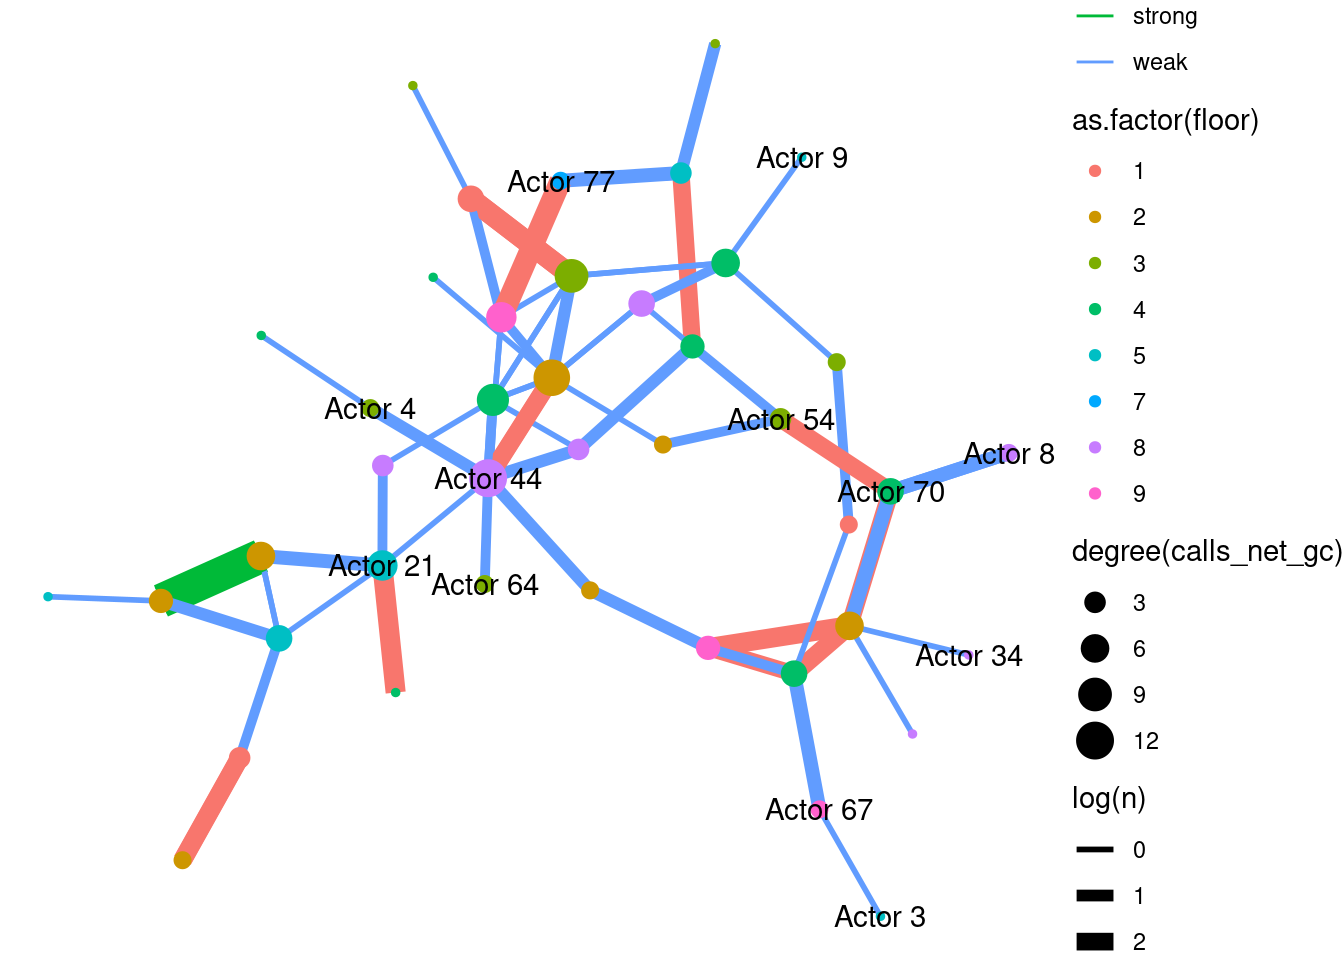
\includegraphics{lab1_files/figure-latex/unnamed-chunk-30-1.pdf}

\begin{Shaded}
\begin{Highlighting}[]
\NormalTok{diamonds }\SpecialCharTok{|}\ErrorTok{\textgreater{}} 
  \CommentTok{\# sample\_frac(0.1) |\textgreater{} }
  \FunctionTok{ggplot}\NormalTok{(}\FunctionTok{aes}\NormalTok{(}\AttributeTok{x =}\NormalTok{ carat, }\AttributeTok{y =}\NormalTok{ price, }\AttributeTok{color =}\NormalTok{ cut))}\SpecialCharTok{+}
  \FunctionTok{geom\_point}\NormalTok{(}\AttributeTok{alpha =} \FloatTok{0.1}\NormalTok{)}\SpecialCharTok{+}
  \FunctionTok{scale\_x\_log10}\NormalTok{()}\SpecialCharTok{+}
  \FunctionTok{scale\_y\_log10}\NormalTok{()}\SpecialCharTok{+}
  \FunctionTok{theme\_minimal}\NormalTok{()}
\end{Highlighting}
\end{Shaded}

\includegraphics{lab1_files/figure-latex/unnamed-chunk-31-1.pdf}

\hypertarget{questions-to-think-about}{%
\subsection{Questions to think about}\label{questions-to-think-about}}

\begin{enumerate}
\def\labelenumi{\arabic{enumi}.}
\tightlist
\item
  What to do if there is too much data?
\item
  Linear regression and age, can you start age at 18 if respondents with
  less age
\item
  What other quantities would be good to logarithmize?
\end{enumerate}

\hypertarget{self-practice}{%
\subsubsection{Self practice}\label{self-practice}}

\begin{enumerate}
\def\labelenumi{\arabic{enumi}.}
\tightlist
\item
  Посчитайте, сколько праздничных дней в каждом году
\item
  Правда ли, что в праздники арендуют больше, чем в обычные дни
\item
  Добавим к праздникам выходные. Правда ли, что в праздники и выходные
  арендуют больше, чем в обычные дни?
\item
  Связано ли количество арендованных велосипедов и температура
\item
  Отличается ли спрос по годам
\item
  Отличается ли спрос по временам года?
\item
  Отличается ли спрос в выходные-не выходные по временам года
\item
  Связано ли количество арендованных велосипедов и влажность?
\end{enumerate}

\hypertarget{hw}{%
\subsection{HW}\label{hw}}

Есть данные и два варианта задания:

\begin{enumerate}
\def\labelenumi{\arabic{enumi}.}
\tightlist
\item
  Повторить картинку. Она странная, и плохая, попробуйте её
  улучшить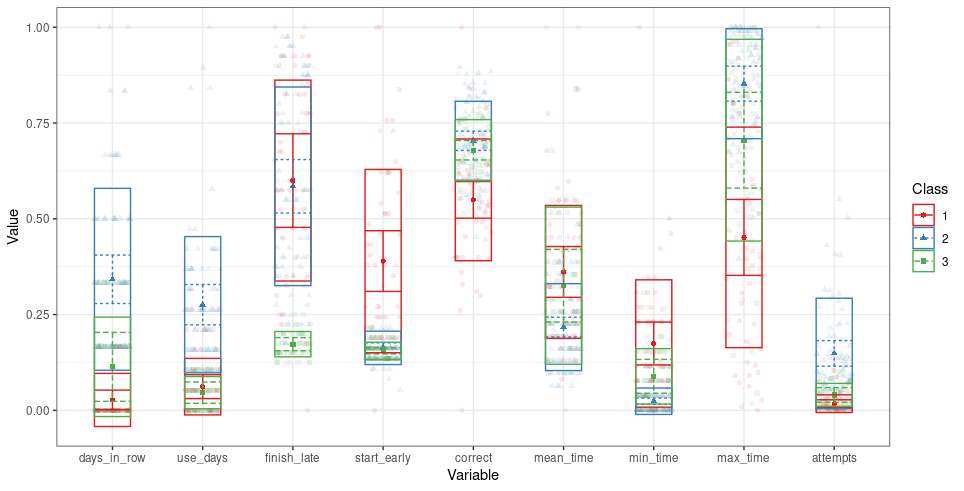
\includegraphics{data/LPA.png}
\item
  С помощью графика\textbackslash графиков показать отличия между 3
  группами студентов, но не рисуйте больше 3 графиков. Представьте, что
  их нужно её в статью пихнуть.
\end{enumerate}

\begin{Shaded}
\begin{Highlighting}[]
\NormalTok{df\_lp }\OtherTok{\textless{}{-}} \FunctionTok{read\_csv}\NormalTok{(}\StringTok{"data/students\_data.csv"}\NormalTok{)}
\end{Highlighting}
\end{Shaded}

\begin{verbatim}
## Rows: 190 Columns: 10
## -- Column specification --------------------------------------------------------
## Delimiter: ","
## chr (1): profile
## dbl (9): days_in_a_row, use_days, finish_late, start_early, correct, mean_ti...
## 
## i Use `spec()` to retrieve the full column specification for this data.
## i Specify the column types or set `show_col_types = FALSE` to quiet this message.
\end{verbatim}

\begin{Shaded}
\begin{Highlighting}[]
\NormalTok{df\_lp }\SpecialCharTok{|}\ErrorTok{\textgreater{}} \FunctionTok{summary}\NormalTok{()}
\end{Highlighting}
\end{Shaded}

\begin{verbatim}
##    profile          days_in_a_row      use_days       finish_late    
##  Length:190         Min.   :0.000   Min.   : 0.000   Min.   : 0.000  
##  Class :character   1st Qu.:2.000   1st Qu.: 2.250   1st Qu.: 3.000  
##  Mode  :character   Median :4.000   Median : 5.000   Median : 7.500  
##                     Mean   :3.547   Mean   : 6.311   Mean   : 8.126  
##                     3rd Qu.:5.000   3rd Qu.:10.000   3rd Qu.:13.000  
##                     Max.   :8.000   Max.   :17.000   Max.   :23.000  
##   start_early        correct         mean_time         min_time    
##  Min.   : 0.000   Min.   :0.2843   Min.   : 0.045   Min.   : 4.70  
##  1st Qu.: 2.000   1st Qu.:0.5244   1st Qu.:20.778   1st Qu.:18.70  
##  Median : 3.000   Median :0.6564   Median :32.465   Median :22.20  
##  Mean   : 4.358   Mean   :0.6731   Mean   :32.917   Mean   :23.28  
##  3rd Qu.: 4.000   3rd Qu.:0.8225   3rd Qu.:43.414   3rd Qu.:27.27  
##  Max.   :20.000   Max.   :0.9987   Max.   :77.436   Max.   :59.50  
##     max_time         attemps      
##  Min.   :  2.70   Min.   :  10.0  
##  1st Qu.: 82.42   1st Qu.: 149.2  
##  Median :110.50   Median : 293.5  
##  Mean   :103.80   Mean   : 611.2  
##  3rd Qu.:132.07   3rd Qu.:1021.0  
##  Max.   :173.90   Max.   :2214.0
\end{verbatim}

Это почти совсем как настоящий датасет из образовательной аналитики. На
одном курсе по юриспруденции в Недерландах студентам предложиди
воспользоваться мобильным приложением, где они могли отвечать на вопросы
про курс и лучше подготовиться к экзамену. Эти данные кластеризовали
каким-то гаусовским алгоритмом и отдали вам для визуализации.

\begin{enumerate}
\def\labelenumi{\arabic{enumi}.}
\tightlist
\item
  \textbf{profile --} выделленый кластер, к которому принадлежат
  студенты
\item
  \textbf{days\_in\_a\_row} -- количество последовательных дней, когда
  использовали приложение
\item
  \textbf{use\_days --} сколько дней приложение использовали всего
\item
  \textbf{finish\_late --} за сколько дней до начала экзамена студенты
  прекратили пользоваться приложением
\item
  \textbf{start\_early --} через сколько дней с начала курса студент
  зашёл в приложение
\item
  \textbf{correct --} процент правильных ответов
\item
  \textbf{mean\_time, min\_time, max\_time --} среднее, минимальное и
  максимально время ответа в приложении
\item
  \textbf{attempts --} насколько вопросов попробовал ответить студент
\end{enumerate}

\hypertarget{additional-materials}{%
\subsection{Additional materials}\label{additional-materials}}

\begin{enumerate}
\def\labelenumi{\arabic{enumi}.}
\tightlist
\item
  Wickham, Hadley. ``A layered grammar of graphics.'' Journal of
  Computational and Graphical Statistics 19, no. 1 (2010): 3-28.
  \url{https://doi.org/10.1198/jcgs.2009.07098}
\end{enumerate}

\end{document}
